%%%%%%%% ICML 2026 EXAMPLE LATEX SUBMISSION FILE %%%%%%%%%%%%%%%%%

\documentclass{article}

% Recommended, but optional, packages for figures and better typesetting:
\usepackage{microtype}
\usepackage{graphicx}
\usepackage{subcaption}
\usepackage{booktabs} % for professional tables
\usepackage{multirow} % for multi-row cells in tables
\usepackage[table,xcdraw]{xcolor} % for table cell colors
\usepackage{colortbl} % for colored table cells

% Define custom colors for table highlighting
\definecolor{bestgreen}{RGB}{198, 239, 206}  % Light green for best results
\definecolor{goodblue}{RGB}{221, 235, 247}   % Light blue for our method
\definecolor{neutralgray}{RGB}{242, 242, 242} % Light gray for baseline

% hyperref makes hyperlinks in the resulting PDF.
% If your build breaks (sometimes temporarily if a hyperlink spans a page)
% please comment out the following usepackage line and replace
% \usepackage{icml2026} with \usepackage[nohyperref]{icml2026} above.
\usepackage{hyperref}


% Attempt to make hyperref and algorithmic work together better:
\newcommand{\theHalgorithm}{\arabic{algorithm}}

% Use the following line for the initial blind version submitted for review:
\usepackage{icml2026}

% For preprint, use
% \usepackage[preprint]{icml2026}

% If accepted, instead use the following line for the camera-ready submission:
% \usepackage[accepted]{icml2026}

\usepackage{amsmath}
\usepackage{amssymb}
\usepackage{mathtools}
\usepackage{amsthm}
\newtheorem*{proposition*}{Proposition}
\newtheorem*{theorem*}{Theorem}
\newtheorem*{lemma*}{Lemma}


% if you use cleveref..
\usepackage[capitalize,noabbrev]{cleveref}

% --- DROP-IN: algorithm packages (needed for Appendix algorithm env) ---
\usepackage{algorithm}
\usepackage{algorithmic}

%%%%%%%%%%%%%%%%%%%%%%%%%%%%%%%%
% THEOREMS
%%%%%%%%%%%%%%%%%%%%%%%%%%%%%%%%
\theoremstyle{plain}
\newtheorem{theorem}{Theorem}[section]
\newtheorem{proposition}[theorem]{Proposition}
\newtheorem{lemma}[theorem]{Lemma}
\newtheorem{corollary}[theorem]{Corollary}
\theoremstyle{definition}
\newtheorem{definition}[theorem]{Definition}
\newtheorem{assumption}[theorem]{Assumption}
\theoremstyle{remark}
\newtheorem{remark}[theorem]{Remark}

% Todonotes is useful during development; simply uncomment the next line
%    and comment out the line below the next line to turn off comments
\usepackage[disable,textsize=tiny]{todonotes}
%\usepackage[textsize=tiny]{todonotes}

% The \icmltitle you define below is probably too long as a header.
% Therefore, a short form for the running title is supplied here:
\icmltitlerunning{Graph-RLHF: Correcting Network-Induced Bias}

\begin{document}

\twocolumn[
  \icmltitle{Graph-RLHF: Correcting Network-Induced Sampling Bias \\
  in Reinforcement Learning from Human Feedback}

  % It is OKAY to include author information, even for blind submissions: the
  % style file will automatically remove it for you unless you've provided
  % the [accepted] option to the icml2026 package.

  % List of affiliations: The first argument should be a (short) identifier you
  % will use later to specify author affiliations Academic affiliations
  % should list Department, University, City, Region, Country Industry
  % affiliations should list Company, City, Region, Country

  % You can specify symbols, otherwise they are numbered in order. Ideally, you
  % should not use this facility. Affiliations will be numbered in order of
  % appearance and this is the preferred way.
  \icmlsetsymbol{equal}{*}

  \begin{icmlauthorlist}
    \icmlauthor{Firstname1 Lastname1}{equal,yyy}
    \icmlauthor{Firstname2 Lastname2}{equal,yyy,comp}
    \icmlauthor{Firstname3 Lastname3}{comp}
    \icmlauthor{Firstname4 Lastname4}{sch}
    \icmlauthor{Firstname5 Lastname5}{yyy}
    \icmlauthor{Firstname6 Lastname6}{sch,yyy,comp}
    \icmlauthor{Firstname7 Lastname7}{comp}
    %\icmlauthor{}{sch}
    \icmlauthor{Firstname8 Lastname8}{sch}
    \icmlauthor{Firstname8 Lastname8}{yyy,comp}
    %\icmlauthor{}{sch}
    %\icmlauthor{}{sch}
  \end{icmlauthorlist}

  \icmlaffiliation{yyy}{Department of XXX, University of YYY, Location, Country}
  \icmlaffiliation{comp}{Company Name, Location, Country}
  \icmlaffiliation{sch}{School of ZZZ, Institute of WWW, Location, Country}

  \icmlcorrespondingauthor{Firstname1 Lastname1}{first1.last1@xxx.edu}
  \icmlcorrespondingauthor{Firstname2 Lastname2}{first2.last2@www.uk}

  % You may provide any keywords that you find helpful for describing your
  % paper; these are used to populate the "keywords" metadata in the PDF but
  % will not be shown in the document
  \icmlkeywords{RLHF, Human Feedback, Graph Neural Networks, Fairness, Social Choice}

  \vskip 0.3in
]

% this must go after the closing bracket ] following \twocolumn[ ...

% This command actually creates the footnote in the first column listing the
% affiliations and the copyright notice. The command takes one argument, which
% is text to display at the start of the footnote. The \icmlEqualContribution
% command is standard text for equal contribution. Remove it (just {}) if you
% do not need this facility.

% Use ONE of the following lines. DO NOT remove the command.
% If you have no special notice, KEEP empty braces:
\printAffiliationsAndNotice{}  % no special notice (required even if empty)
% Or, if applicable, use the standard equal contribution text:
% \printAffiliationsAndNotice{\icmlEqualContribution}

\begin{abstract}
  Reinforcement learning from human feedback (RLHF) typically treats
  annotators as an i.i.d.\ population, ignoring the social, institutional,
  or spatial networks that connect them. We show that when feedback is
  collected through network-based processes (e.g., platform recruitment,
  respondent-driven sampling), standard RLHF implicitly optimizes a
  degree-weighted social welfare that over-represents structurally
  central communities. To address this, we propose \textsc{Graph-RLHF}, a
  framework that models annotators as nodes in a graph and corrects for
  network-induced sampling bias. Our approach combines a graph-personalized
  reward model that shares information across neighboring annotators with a
  graph-balanced aggregation scheme that reweights feedback to approximate a
  designer-chosen welfare target. We provide theoretical guarantees showing
  that Graph-RLHF recovers the target welfare under exact debiasing, and
  otherwise optimizes an induced welfare with deviation bounded by the
  $\ell_1$ distance between induced and target weight distributions.
  Experiments on synthetic graphs and a real-world global preference dataset
  demonstrate up to 29\% improvement in alignment accuracy and 74\% reduction
  in cross-region disparity. Our framework is compatible with existing RLHF
  and DPO pipelines, offering a principled way to control whose preferences
  an aligned model encodes.
\end{abstract}

\section{Introduction}
\label{sec:intro}

Reinforcement learning from human feedback (RLHF) has become a central paradigm for aligning large language models and other AI systems with human preferences and norms.
The now-standard pipeline---supervised fine-tuning, preference-based reward modeling, and reinforcement learning or direct preference optimization---has been popularized by work such as InstructGPT~\citep{ouyang2022instructgpt} and formalized and surveyed in recent overviews of RLHF for language models~\citep{kaufmann2025survey,lambert2025rlhfbook}.
Recent advances such as Direct Preference Optimization (DPO)~\citep{rafailov2023dpo} and RL from AI feedback (RLAIF)~\citep{lee2024rlaif} have further scaled and simplified this pipeline, enabling alignment at web scale using variants of pairwise preference data.
Across these methods, human feedback is typically treated as an i.i.d.\ sample from an abstract population of annotators: individual raters may have different noise levels, but the population itself is assumed to be unstructured.

Prior work has addressed preference heterogeneity through personalized RLHF~\citep{poddar2024vpl}, group-robust methods~\citep{chakraborty2024maxminrlhf,ramesh2024grpo}, and social choice theory~\citep{ge2024axioms,dai2024mapping,conitzer2024socialchoice}.
Recent datasets such as Collective Alignment~\citep{openai2025ca1} collect globally distributed feedback with rich demographics, revealing significant geographic imbalance in annotator pools. However, these approaches treat annotators as independent samples from predefined categories rather than as nodes in a network.
Meanwhile, network sampling research~\citep{wejnert2010rds,lerman2016majorityillusion,saxena2024fairsna,dong2021edits} shows that graph structure profoundly affects who is sampled and represented. We bridge these literatures by explicitly modeling the network structure governing recruitment, showing that standard RLHF implicitly optimizes a degree-weighted welfare. Full related work is in Appendix~\ref{sec:related}.

Despite these insights, current RLHF practice implicitly assumes that feedback providers are drawn i.i.d.\ from a homogeneous pool.
In reality, RLHF data collection often happens through platforms and institutions that are themselves networked: crowdworkers recruited through peer networks, users of a single social platform, students or teachers within an educational institution, or residents connected through urban infrastructure.
When preference data are collected from such populations, they are effectively network samples---more akin to respondent-driven or snowball sampling than to simple random sampling.
Ignoring this structure means that standard RLHF pipelines may inadvertently align models to the preferences of structurally central communities: those with many connections, high platform activity, or privileged institutional positions.
This raises concerns for domains where AI systems mediate social interaction, education, and urban services: whose values are being encoded, and whose are being marginalized?


\begin{figure*}[t]
    \centering
    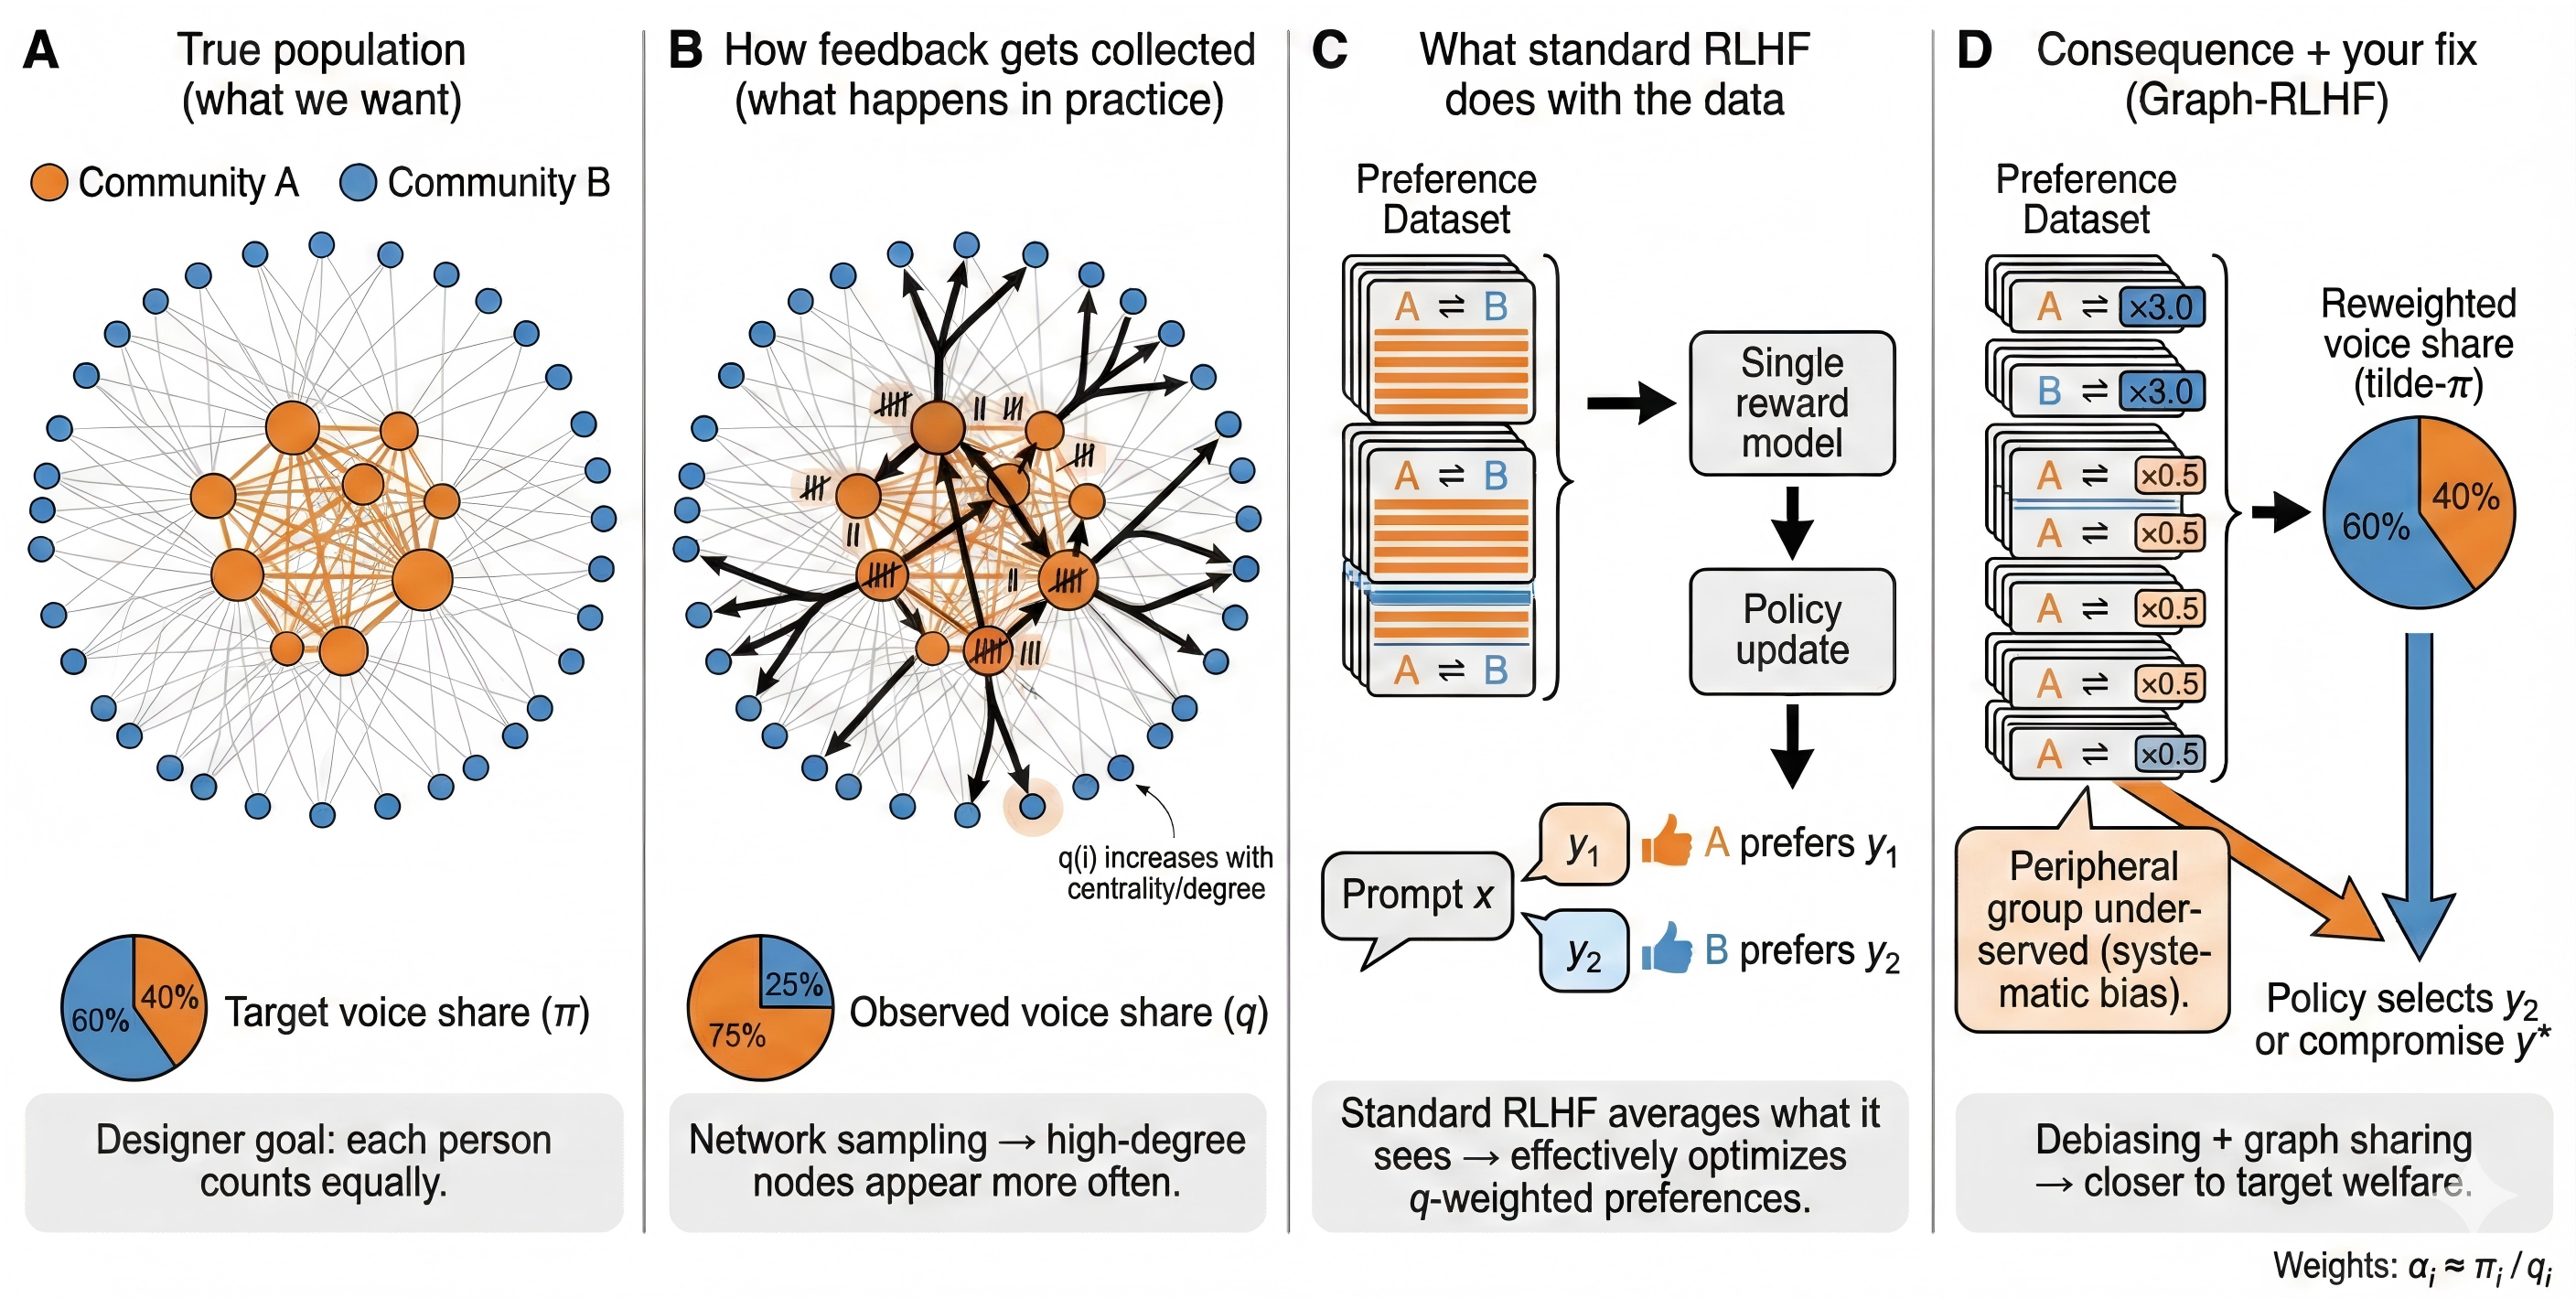
\includegraphics[width=0.8\linewidth]{figures/network_bias.png}
    \caption{Network-induced sampling bias in RLHF. (A) Annotators form a network with communities; the designer’s target is a normative voice distribution $\pi$ (e.g., equal-per-person). (B) Feedback collected via network processes (random-walk / snowball / platform exposure) over-samples high-degree nodes, producing an observed inclusion distribution $q$ skewed toward central communities. (C) Standard RLHF ignores annotator identity and trains on the marginal data, implicitly optimizing the $q$-weighted aggregate preference. (D) Graph‑RLHF corrects this by (i) sharing information across neighbors in a graph-personalized reward model and (ii) reweighting feedback using $\alpha_i$ to approximate $\pi$, yielding an induced distribution $\tilde\pi$ closer to the target.}
    \label{fig:network-bias}
\end{figure*}

Our work addresses this gap by treating feedback providers as nodes in a graph. We propose Graph-RLHF, which models the network connecting annotators and uses this structure to regularize per-annotator rewards and correct for network-induced sampling bias.

\paragraph{Contributions.}
We (i) formalize networked RLHF and show naive pipelines optimize a $q$-weighted welfare,
(ii) propose Graph-RLHF (graph-personalized reward + graph-balanced aggregation),
(iii) instantiate importance-weighted RM and Graph-DPO/RLHF objectives,
(iv) prove the induced-welfare view with error controlled by $\|\tilde\pi-\pi\|_1$,
and (v) validate on synthetic graphs and a real-world global preference dataset, demonstrating up to 29\% improvement in alignment and 74\% reduction in cross-region disparity.

%%%%%%%%%%%%%%%%%%%%%%%%%%%%%%%%%%%%%%%%%%%%%%%%%%%%%%%%%%%%%%%%%%%%%%%%%%%%%%%
%%%%%%%%%%%%%%%%%%%%%%%%%%%%%%%%%%%%%%%%%%%%%%%%%%%%%%%%%%%%%%%%%%%%%%%%%%%%%%%

\section{Problem Formulation}
\label{sec:problem}

We consider reinforcement learning from human feedback (RLHF) in settings where
humans providing feedback are embedded in an underlying social, institutional,
or spatial network. Our goal is to make explicit (i) how such network structure
affects which preferences are observed, and (ii) how this interacts with
the social welfare notion that RLHF implicitly optimizes.

\subsection{Human Feedback and Policies}

Let $\mathcal{X}$ denote the space of inputs (e.g., prompts) and $\mathcal{Y}_x$
the set of outputs available for input $x \in \mathcal{X}$. A (stochastic)
policy $\pi_\phi$ with parameters $\phi$ defines a conditional distribution
$\pi_\phi(y \mid x)$ over outputs $y \in \mathcal{Y}_x$.

Human feedback is collected in the form of pairwise preferences over candidate
outputs. Concretely, we observe a dataset
\begin{equation}
    \mathcal{D}
    =
    \left\{ (x_t, y_t^+, y_t^-, i_t) \right\}_{t=1}^T,
\end{equation}
where $x_t \in \mathcal{X}$ is an input, $y_t^+, y_t^- \in \mathcal{Y}_{x_t}$ are
two candidate outputs, and $i_t \in V$ is the identity of the human annotator
who provided the preference $y_t^+ \succ y_t^-$.\footnote{We restrict to
pairwise comparison for clarity. Extension to graded feedback or top-$k$ lists
is straightforward.}

We write $\mathcal{I} = V$ for the set of annotators or stakeholders who may
provide feedback. In standard RLHF training, $i_t$ is recorded but then
discarded in downstream modeling; we keep it explicit.

\subsection{Networked Annotators}
\label{subsec:networked-annotators}

We model annotators as nodes in a graph capturing social, institutional, or
spatial relationships.

\begin{definition}[Annotator graph]
Let $G = (V, E)$ be an undirected graph, where $V = \mathcal{I}$ is the set of
annotators and $E \subseteq V \times V$ encodes relationships (e.g., social
ties, class membership, shared institution, spatial adjacency). We write
$d_i = \deg(i)$ for the degree of node $i$ and $N(i)$ for its neighbors.
\end{definition}

The graph $G$ is not assumed to be fully observed or perfectly accurate in
practice; in our experiments we instantiate $G$ using explicit
ties (when available) or similarity between annotators (e.g., demographic or
preference similarity).

Importantly, the feedback collection process is often graph-structured: platforms over-sample active users, recruitment spreads via social ties, and institutions contribute proportionally to size. We capture this by modeling $i_t$ as drawn from a graph-dependent distribution $q$ (see Appendix~\ref{app:problem-details} for extensions to graph uncertainty). Figure~\ref{fig:network-bias} illustrates the problem and our solution.
\begin{definition}[Inclusion probabilities]
\label{def:inclusion-prob}
At each feedback event $t$, the annotator index $i_t$ is sampled from a fixed
distribution $q(\cdot)$ on $V$, which we call the inclusion
distribution. We denote $q_i = q(i)$, so that
$\sum_{i \in V} q_i = 1$, and write
\begin{equation}
    i_t \sim q(\cdot),
    \quad
    (x_t, y_t^+, y_t^-) \sim \mathcal{T}(i_t),
\end{equation}
where $\mathcal{T}$ is a task-dependent distribution over prompts and
candidates conditioned on annotator $i_t$.
\end{definition}

In practice $q$ is often unknown but approximately proportional to graph centrality (e.g., degree or PageRank); see Appendix~\ref{app:network-bias} Appendix~\ref{app:problem-details} for contextual inclusion extensions.

\subsection{Individual Utilities and Social Welfare}
\label{subsec:utilities-welfare}

We assume each annotator $i$ has a latent utility function or
preference over model outputs.

\begin{definition}[Individual utilities]
For each annotator $i \in V$, we define a utility function
$u_i : \mathcal{X} \times \mathcal{Y}_x \to \mathbb{R}$, where
$u_i(x,y)$ measures the (unobserved) desirability of model output $y$ for input
$x$ according to $i$. We assume that observed preferences are consistent with
these utilities, e.g.\ under a logistic choice model,
\begin{equation}
\begin{aligned}
    \Pr\!\left( y^+ \succ y^- \mid x, i \right)
    =
    \sigma\!\left( s_i \cdot (u_i(x,y^+) - u_i(x,y^-)) \right), \\
    s_i > 0,
\end{aligned}
\end{equation}
where $\sigma(\cdot)$ is the logistic sigmoid and $s_i > 0$ is a
rater-specific scale (or inverse temperature) capturing how
``strict'' annotator $i$ is in their comparisons.
\end{definition}

Given a policy $\pi_\phi$, annotator $i$'s expected utility is
\begin{equation}
    U_i(\pi_\phi)
    =
    \mathbb{E}_{x \sim p_{\text{data}},\, y \sim \pi_\phi(\cdot \mid x)}
    \left[ u_i(x,y) \right],
\end{equation}
where $p_{\text{data}}$ is the distribution of inputs.

RLHF, implicitly or explicitly, optimizes a social welfare function
which aggregates these individual utilities into a scalar objective.

\begin{definition}[Target social welfare]
\label{def:target-welfare}
We consider linear social welfare functions of the form
\begin{equation}
    W_{\text{target}}(\pi_\phi)
    \;=\;
    \sum_{i \in V} \pi_i \, U_i(\pi_\phi),
    \quad
    \pi_i \ge 0,
    \quad
    \sum_{i \in V} \pi_i = 1,
    \label{eq:target-welfare}
\end{equation}
where $\pi = (\pi_i)_{i \in V}$ are normative weights expressing whose
utilities should matter and how much.
\end{definition}

Two canonical choices are equal-per-person ($\pi_i = 1/|V|$) and equal-per-community ($\pi_i = 1/(K|C_k|)$ for $i \in C_k$). More complex weightings fit naturally into \eqref{eq:target-welfare}.

\subsection{What Standard RLHF Optimizes}
\label{subsec:standard-rlhf}

In standard RLHF and DPO pipelines, annotator identity is discarded and a
single scalar reward model $r_\theta(x,y)$ is fit to preferences generated by
the data collection process. Regardless of whether the underlying preference
mechanism is a mixture over annotators, the population objective
optimized by this pipeline is defined by the marginal preference distribution
induced by sampling $i \sim q$.

To connect this to welfare, we adopt the following assumption, which is
standard in analyses of scalar Bradley--Terry reward modeling:

\begin{assumption}[Scalar population reward under $q$]
\label{ass:scalar-q}
There exists a scalar function $r_q^\star(x,y)$ such that for all
$x, y^+, y^-$,
\begin{equation}
    \Pr(y^+ \succ y^- \mid x)
    =
    \sigma\!\big(r_q^\star(x,y^+) - r_q^\star(x,y^-)\big),
    \label{eq:scalar-q-reward}
\end{equation}
where the probability on the left-hand side is taken over the data-generating
process that samples $i \sim q$ and then draws a comparison from
$\mathcal{T}(i)$.
\end{assumption}

Under Assumption~\ref{ass:scalar-q}, maximum-likelihood reward modeling that
ignores annotator identity is consistent for $r_q^\star$ (up to an additive
constant), and subsequent policy optimization maximizes
$\mathbb{E}_{x, y \sim \pi_\phi}[r_q^\star(x,y)]$.

In settings where each annotator's utility $u_i(x,y)$ is on a comparable scale
and the scalar $r_q^\star$ can be interpreted as an aggregate of individual
utilities, the induced objective corresponds to the $q$-weighted welfare
\begin{equation}
    W_{\text{obs}}(\pi_\phi)
    =
    \sum_{i \in V} q_i \, U_i(\pi_\phi).
    \label{eq:obs-welfare}
\end{equation}

When preference heterogeneity is small, the marginal can be approximated by a single logistic model (see Appendix~\ref{app:proof-mixture} for a formal bound). Even when heterogeneity is large, Graph-RLHF can be interpreted via induced weights (Section~\ref{subsec:theory-unbiased}).

Our goal in the remainder of the paper is to correct the mismatch between
the observed welfare $W_{\text{obs}}$ (weighted by inclusion $q$) and the
desired target welfare $W_{\text{target}}$ (weighted by normative $\pi$).
When feedback is collected via networked processes where $q_i$ correlates with
graph centrality (e.g., $q_i \propto d_i$), \eqref{eq:obs-welfare}
systematically over-weights central communities.

\subsection{Network-Induced Misalignment}
\label{subsec:misalignment}

We can now formalize the misalignment induced by standard RLHF as the
difference between the observed social welfare \eqref{eq:obs-welfare}
and the target welfare \eqref{eq:target-welfare}.

\begin{definition}[Network-induced misalignment]
Given inclusion weights $q = (q_i)$ and normative weights $\pi = (\pi_i)$, we
define the network-induced misalignment of a policy $\pi_\phi$ as
\begin{equation}
    \Delta(\pi_\phi)
    =
    W_{\text{target}}(\pi_\phi)
    -
    W_{\text{obs}}(\pi_\phi)
    =
    \sum_{i \in V} (\pi_i - q_i) \, U_i(\pi_\phi).
    \label{eq:misalignment}
\end{equation}
\end{definition}

When $\pi = q$, the observed and target welfare coincide and standard RLHF is
well-aligned by construction. When $\pi \neq q$, the RLHF pipeline optimizes
$W_{\text{obs}}$ while our normative objective is $W_{\text{target}}$, leading
to systematic bias. In many realistic settings we expect
\begin{equation}
    q_i \propto \text{centrality}_G(i)
    \quad\text{and}\quad
    \pi_i \in \left\{ \tfrac{1}{|V|},\ \tfrac{1}{K|C_k|}, \ldots \right\},
\end{equation}
so that graph-central annotators are over-weighted relative to the desired
welfare.

We are particularly interested in misalignment across communities in the annotator graph, measured by dispersion across community-level welfares (see Appendix~\ref{app:problem-details} for formal definitions).

\subsection{Goal: Graph-Aware RLHF}
\label{subsec:goal}

Our goal is to design an RLHF procedure that learns a graph-consistent reward model and trains a policy $\pi_\phi$ optimizing the induced welfare $\widetilde{W}(\pi_\phi) = \sum_i \tilde\pi_i U_i(\pi_\phi)$, where $\tilde\pi \approx \pi$. We seek to reduce network-induced misalignment in \eqref{eq:misalignment} while maintaining strong overall performance.

%%%%%%%%%%%%%%%%%%%%%%%%%%%%%%%%%%%%%%%%%%%%%%%%%%%%%%%%%%%%%%%%%%%%%%%%%%%%%%%
%%%%%%%%%%%%%%%%%%%%%%%%%%%%%%%%%%%%%%%%%%%%%%%%%%%%%%%%%%%%%%%%%%%%%%%%%%%%%%%


\section{Method}
\label{sec:method}

\textsc{Graph-RLHF} augments standard RLHF with three components:
\textbf{(1) Graph-personalized reward modeling (GPRM):} learn $r_\theta(x,y,i) \approx u_i(x,y)$ via graph encoder + Laplacian smoothness.
\textbf{(2) Graph-balanced aggregation (GBA):} compute importance weights $\alpha_i = \pi_i / \hat q_i$ to define induced welfare $\tilde\pi_i = \hat q_i \alpha_i$.
\textbf{(3) Graph-weighted DPO/RLHF:} reweight preferences by $\alpha_i$ to align policy with target welfare.

\textbf{Notation:} $\pi_\phi$ = policy; $\pi_i$ = welfare weight of annotator $i$; $q$ = inclusion distribution; $\alpha$ = importance weights; $\tilde\pi = q \odot \alpha$ = induced welfare.
We focus on DPO; see Appendix~\ref{app:ppo} for RLHF with explicit reward.

\begin{figure*}[t]
    \centering
    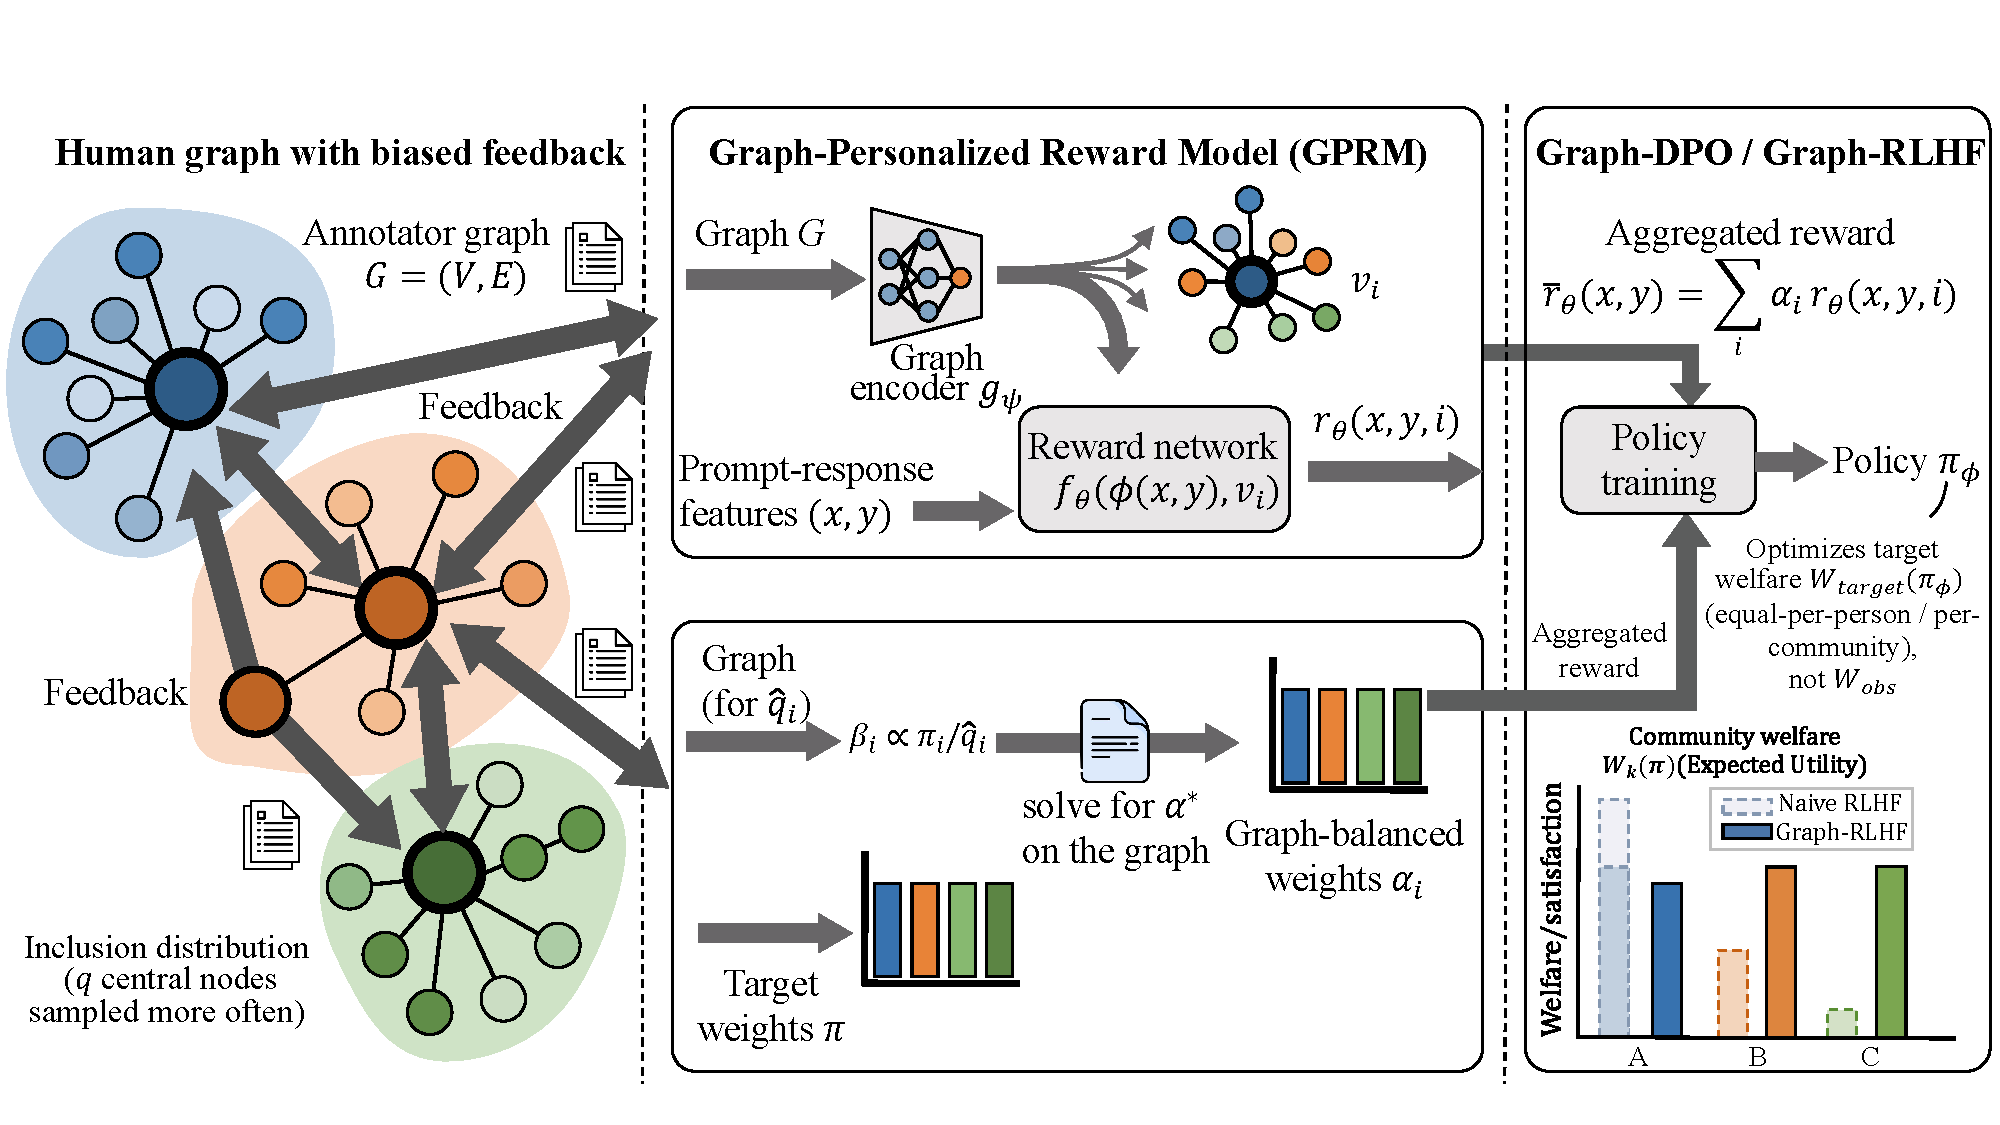
\includegraphics[width=0.75\textwidth]{figures/method figure.pdf}
    \caption{\textbf{Overview of \textsc{Graph-RLHF}.} Left: annotator graph $G$ with network-biased sampling. Middle: GPRM learns per-annotator rewards $r_\theta(x,y,i)$; GBA computes importance weights $\alpha_i$ to define induced welfare $\tilde\pi$. Right: Graph-DPO trains policy against target welfare rather than network-induced welfare.}
    \label{fig:graph-rlhf-overview}
\end{figure*}


\subsection{Graph-Personalized Reward Model (GPRM)}
\label{subsec:gprm}

The first component of \textsc{Graph-RLHF} is a per-annotator reward model
that leverages the annotator graph $G$ to share statistical strength and
encourage locally smooth preferences.

\paragraph{Annotator embeddings from the graph.}

Each annotator $i \in V$ is associated with an initial feature vector
$h_i \in \mathbb{R}^{d_0}$ (e.g., demographic attributes, interaction
statistics, or a learned ID embedding). We pass $\{h_i\}$ through a graph
encoder $g_\psi$ defined on $G$ to obtain annotator embeddings
$v_i \in \mathbb{R}^d$:
\begin{equation}
    v_i = g_\psi(i; G, \{h_j\}_{j \in V}),
    \qquad i \in V,
\end{equation}
where $g_\psi$ can be any differentiable message-passing network (e.g., a GCN
or GraphSAGE). We denote by $\mathbf{V} \in \mathbb{R}^{|V| \times d}$ the
matrix that stacks all embeddings row-wise.

\paragraph{Reward network.}

For each input--output pair $(x,y)$ we compute a representation
$\phi(x,y) \in \mathbb{R}^{d_x}$, for example by extracting hidden states from
a frozen base language model and optionally passing them through a small MLP.
The graph-personalized reward model is then defined as
\begin{equation}
    r_\theta(x,y,i)
    =
    f_\theta(\phi(x,y), v_i),
    \label{eq:gprm}
\end{equation}
where $f_\theta$ is a small neural network (e.g., a two-layer MLP) with
parameters $\theta$ that maps the concatenated features
$[\phi(x,y); v_i]$ to a scalar reward.

Intuitively, $r_\theta(x,y,i)$ plays the role of an amortized estimator for
the latent utility $u_i(x,y)$ introduced in
Section~\ref{subsec:utilities-welfare}.

\paragraph{Scale prediction.}
To model rater-specific strictness, we predict a per-annotator scale
\begin{equation}
    s_i = \exp(g_\xi(v_i)),
    \label{eq:scale}
\end{equation}
where $g_\xi$ is a small MLP with parameters $\xi$.

\paragraph{Graph-regularized preference loss.}

Given the preference dataset
$\mathcal{D} = \{(x_t, y_t^+, y_t^-, i_t)\}_{t=1}^T$, we define a
graph-regularized Bradley--Terry loss
\begin{align}
    \mathcal{L}_{\text{GPRM}}(\theta, \psi, \xi)
    =
    - \sum_{t=1}^T
    \alpha_{i_t}^\star \,
    \log \sigma\Big(
        s_{i_t} \big[
        r_\theta(x_t, y_t^+, i_t) \nonumber \\
        -
        r_\theta(x_t, y_t^-, i_t)
        \big]
    \Big)
    + \lambda_v \, \mathrm{Tr}(\mathbf{V}^\top L_w \mathbf{V}) \nonumber \\
    + \lambda_s \sum_{i \in V} \pi_i (\log s_i)^2
    + \lambda_\theta \|\theta\|_2^2,
    \label{eq:gprm-loss}
\end{align}
Here $\alpha_{i_t}^\star \ge 0$ are importance weights (Section~\ref{subsec:gba}), $L_w$ is the weighted Laplacian encouraging local smoothness, and $\lambda_v, \lambda_s, \lambda_\theta$ are regularization hyperparameters. The importance weights correct for the mismatch between $q$ and $\pi$: choosing $\alpha_i = \pi_i / q_i$ makes the weighted loss behave as if annotators were sampled from $\pi$. See Appendix~\ref{app:method-details} for details on over-smoothing and heterophily.

\subsection{Graph-Balanced Aggregation (GBA)}
\label{subsec:gba}

The second component of \textsc{Graph-RLHF} is a procedure that computes
importance weights $\alpha_i$ from estimated inclusion probabilities
$\hat q_i$ and normative weights $\pi_i$. These weights serve two roles:

\begin{enumerate}
    \item They enter the GPRM loss \eqref{eq:gprm-loss} as reweighting
    coefficients on $q$-sampled data, correcting for network-induced sampling
    bias.
    \item They define an induced welfare distribution
    $\tilde\pi_i := \hat q_i \alpha_i$ and an aggregated reward
    $\bar r_\theta(x,y) = \sum_{i \in V} \tilde\pi_i \, r_\theta(x,y,i)$ that
    approximates the target welfare.
\end{enumerate}

\paragraph{Estimating inclusion probabilities.}

For each annotator $i \in V$ we estimate an inclusion probability
$\hat q_i$, which approximates how likely $i$ is to contribute feedback under
the data collection process. When per-annotator sample counts $n_i$ are
available, a direct estimator is $\hat q_i = n_i / \sum_j n_j$. In settings
where the sampling mechanism is not directly observed, a degree-based
estimator is
\begin{equation}
    \hat q_i
    =
    \frac{d_i^\gamma}{\sum_{j \in V} d_j^\gamma},
    \qquad
    \gamma \in [0,1],
    \label{eq:qhat}
\end{equation}
where $\gamma = 0$ corresponds to assuming uniform sampling and
$\gamma = 1$ approximates random-walk or respondent-driven sampling, which
oversamples high-degree nodes. Degree-based estimators are useful when $n_i$
is unavailable or when extrapolating beyond observed annotators.

We recommend $\gamma = 0.5$ as a default; see Appendix~\ref{app:method-details} for guidance on choosing $\gamma$.

\paragraph{Raw importance weights.}

Given target welfare weights $\pi$ and inclusion estimates $\hat q$, define
the raw (unnormalized) importance weight for annotator $i$ as
\begin{equation}
    \tilde\alpha_i
    =
    \frac{\pi_i}{\hat q_i + \varepsilon},
    \label{eq:alpha-raw}
\end{equation}
where $\varepsilon > 0$ is a small constant for numerical stability.

\paragraph{Graph-regularized importance weights.}

The raw ratio $\tilde\alpha_i$ can be noisy and may not respect additional
fairness or smoothness desiderata. We therefore compute regularized
importance weights $\alpha$ by solving
\begin{equation}
\begin{aligned}
    \alpha^\star
    = \arg\min_{\alpha \in \mathbb{R}^{|V|}}
    \Bigg\{
        \frac{1}{2} \|\alpha - \tilde\alpha\|_2^2
        + \lambda_{\text{smooth}} \, \alpha^\top L_w \alpha \\
        + \lambda_{\text{comm}} \sum_{k=1}^{K}
          \Big( \sum_{i \in C_k} \hat q_i \alpha_i - \rho_k \Big)^2
        + \lambda_{\text{var}} \sum_{i \in V} \hat q_i \alpha_i^2
    \Bigg\}
    \\
    \text{s.t.}\quad
    \alpha_i \ge 0 \ \forall i \in V,
    \quad
    \sum_{i \in V} \hat q_i \alpha_i = 1,
\end{aligned}
\label{eq:alpha-star}
\end{equation}
where $\rho_k$ are desired community masses. The first term keeps $\alpha$ close to raw weights; the Laplacian enforces smoothness; the community term controls representation; and $\lambda_{\text{var}}$ controls variance/ESS. See Appendix~\ref{app:wstar-details} for details.

\paragraph{Aggregated reward.}

Define the induced welfare weights $\tilde\pi_i := \hat q_i \alpha_i^\star$.
We aggregate personalized rewards as
\begin{equation}
    \bar r_\theta(x,y)
    =
    \sum_{i \in V} \tilde\pi_i \, r_\theta(x,y,i)
    =
    \sum_{i \in V} \hat q_i \alpha_i^\star \, r_\theta(x,y,i).
    \label{eq:aggregated-reward}
\end{equation}
When $\hat q \approx q$ and $\alpha^\star \approx \pi / q$, we have
$\tilde\pi \approx \pi$, and the aggregated reward approximates the target.

When $|V|$ is large, $\bar r_\theta$ can be approximated by Monte Carlo (see Appendix~\ref{app:method-details} for details). In Graph-DPO, preferences are reweighted directly by $\alpha_{i_t}^\star$.

\subsection{Graph-Weighted DPO and RLHF}
\label{subsec:graph-dpo}

The final component of \textsc{Graph-RLHF} is a policy optimization objective
that incorporates the graph-balanced weights. We describe a DPO-style
objective here; RLHF with an explicit reward model is covered in
Appendix~\ref{app:ppo}.

\paragraph{Graph-weighted DPO.}

Direct Preference Optimization (DPO) aligns a policy $\pi_\phi$ to observed
preferences by comparing log-probabilities under $\pi_\phi$ and a fixed
reference policy $\pi_{\text{ref}}$. For a preference pair
$(x_t, y_t^+, y_t^-, i_t)$, the standard DPO loss is
\begin{equation}
\begin{aligned}
    \ell_{\text{DPO}}(\phi; x_t, y_t^+, y_t^-)
    =
    - \log \sigma\Big(
        \beta \big[
        \log \pi_\phi(y_t^+ \mid x_t) \qquad \\ - \log \pi_\phi(y_t^- \mid x_t)
        - \log \pi_{\text{ref}}(y_t^+ \mid x_t)
        + \log \pi_{\text{ref}}(y_t^- \mid x_t)
        \big]
    \Big),
    \label{eq:dpo}
\end{aligned}
\end{equation}
where $\beta > 0$ is a temperature parameter.

We define the graph-weighted DPO objective as
\begin{equation}
    \mathcal{L}_{\text{Graph-DPO}}(\phi)
    =
    \sum_{t=1}^T
    \alpha_{i_t}^\star \,
    \ell_{\text{DPO}}(\phi; x_t, y_t^+, y_t^-),
    \label{eq:graph-dpo}
\end{equation}
where $\alpha_{i_t}^\star$ are the importance weights computed in
Section~\ref{subsec:gba}. At the population level, weighting by
$\alpha_i^\star$ converts expectations over $i \sim q$ into expectations
under the induced weights $\tilde\pi = \hat q \odot \alpha^\star$.
Intuitively, each preference is reweighted so that annotators whose voices
should count more in the target welfare---and/or who were under-sampled in
the data---have larger influence on the learned policy.

At the population level, importance weighting converts expectations over $q$ to expectations under $\tilde\pi = q \odot \alpha$ (see Lemma~\ref{lem:graph-dpo-reweight} in Section~\ref{sec:theory}).

\paragraph{Reward-model-based Graph-RLHF.}

Alternatively, we can use the aggregated reward $\bar r_\theta(x,y)$ in a
reward-based RLHF pipeline (e.g., PPO). In that case, $\bar r_\theta$ replaces
the usual scalar reward model in the advantage computation, while the policy
update (e.g., PPO clipping) remains unchanged. Because $\bar r_\theta$ is constructed from the induced welfare weights
$\tilde\pi_i = \hat q_i \alpha_i^\star$, the resulting policy is pushed
toward maximizing the induced welfare $\widetilde{W}$ (which approximates
$W_{\text{target}}$) rather than $W_{\text{obs}}$. See Appendix~\ref{app:ppo} for details.

\paragraph{Graph-Active Feedback.}
For iterative feedback collection, \textsc{Graph-RLHF} suggests an active strategy that queries annotators to reduce network-induced misalignment most efficiently, balancing disagreement, under-representation, and community coverage. See Appendix~\ref{app:active} for details.

%%%%%%%%%%%%%%%%%%%%%%%%%%%%%%%%%%%%%%%%%%%%%%%%%%%%%%%%%%%%%%%%%%%%%%%%%%%%%%%
%%%%%%%%%%%%%%%%%%%%%%%%%%%%%%%%%%%%%%%%%%%%%%%%%%%%%%%%%%%%%%%%%%%%%%%%%%%%%%%


\section{Theoretical Analysis}
\label{sec:theory}

We now analyze network-induced bias in standard RLHF and study how
Graph-RLHF alters the underlying optimization objective. At a high level, we
show that:
(i) standard RLHF (which ignores annotator identity) optimizes a social
welfare weighted by the inclusion distribution $q$ rather than the target
weights $\pi$;
(ii) the importance weights in our graph-personalized reward model align the
population loss with the target distribution; and
(iii) the graph-balanced aggregation scheme enforces community-level fairness
constraints and bounds misalignment across communities.

We work at the level of population objectives and gradients, abstracting away
finite-sample effects and optimization noise. Full proofs and technical
conditions are provided in Appendix~\ref{app:theory-details}.

\subsection{Population Losses and Gradients}

We first formalize the population-level objectives optimized by standard RLHF
and Graph-RLHF. For simplicity, we focus on the reward-modeling stage; the
policy optimization stage follows by standard arguments that connect reward
maximization to social welfare~\citep{kaufmann2025survey}.

Recall the data-generating process from
Section~\ref{sec:problem}: at each step we sample an annotator $i \sim q$,
then sample a preference pair $(x,y^+,y^-) \sim \mathcal{T}(i)$, and observe
the event $y^+ \succ y^-$. Let
$\ell(\theta; x,y^+,y^-,i)$ be the (per-example) Bradley--Terry loss for a
reward model $r_\theta(x,y,i)$:
\begin{equation}
    \ell(\theta; x,y^+,y^-,i)
    =
    - \log \sigma\big(
        r_\theta(x,y^+,i) - r_\theta(x,y^-,i)
    \big).
    \label{eq:bt-loss}
\end{equation}

\paragraph{Standard RLHF.}
The population loss for a scalar reward model
$r_\theta(x,y)$ that ignores annotator identity is
\begin{equation}
    \mathcal{L}_{\text{naive}}(\theta)
    =
    \mathbb{E}_{i \sim q}
    \mathbb{E}_{(x,y^+,y^-) \sim \mathcal{T}(i)}
    \Big[
        \ell_{\text{naive}}(\theta; x,y^+,y^-)
    \Big],
    \label{eq:naive-pop-loss}
\end{equation}
where $\ell_{\text{naive}}$ is obtained from Eq.~\eqref{eq:bt-loss} by
replacing $r_\theta(x,y,i)$ with $r_\theta(x,y)$.
The gradient of $\mathcal{L}_{\text{naive}}$ can be written as
\begin{equation}
\begin{aligned}
    \nabla_\theta \mathcal{L}_{\text{naive}}(\theta)
    =
    \sum_{i \in V} q_i \, g_i(\theta), \qquad\qquad \\
    g_i(\theta)
    :=
    \mathbb{E}_{(x,y^+,y^-) \sim \mathcal{T}(i)}
    [
        \nabla_\theta \ell_{\text{naive}}(\theta; x,y^+,y^-)
    ].
    \label{eq:naive-grad}
\end{aligned}
\end{equation}
Thus standard RLHF performs gradient descent on a $q$-weighted mixture of
per-annotator losses.

\paragraph{Graph-RLHF.}
In Graph-RLHF, the graph-personalized reward model $r_\theta(x,y,i)$ is
trained with importance weights $\alpha_i$ as in
Eq.~\eqref{eq:alpha-raw}, giving population loss
\begin{equation}
    \mathcal{L}_{\text{GPRM}}^{\text{pop}}(\theta)
    =
    \mathbb{E}_{i \sim q}
    \mathbb{E}_{(x,y^+,y^-) \sim \mathcal{T}(i)}
    \Big[
        \alpha_i \, \ell(\theta; x,y^+,y^-,i)
    \Big].
    \label{eq:gprm-pop-loss}
\end{equation}
The corresponding gradient is
\begin{equation}
\begin{aligned}
    \nabla_\theta \mathcal{L}_{\text{GPRM}}^{\text{pop}}(\theta)
    =
    \sum_{i \in V} q_i \alpha_i \, h_i(\theta),
    \qquad\quad \\
    h_i(\theta)
    :=
    \mathbb{E}_{(x,y^+,y^-) \sim \mathcal{T}(i)}
    [
        \nabla_\theta \ell(\theta; x,y^+,y^-,i)
    ].
    \label{eq:gprm-pop-grad}
\end{aligned}
\end{equation}
By Lemma~\ref{lem:iw-identity}, choosing $\alpha_i = \pi_i / q_i$ makes
$\sum_i q_i \alpha_i h_i(\theta) = \sum_i \pi_i h_i(\theta)$, effectively
replacing the sampling distribution $q$ by the target $\pi$.

\subsection{Network Bias in Standard RLHF}

We now show that, under mild conditions, standard RLHF optimizes a welfare
objective weighted by $q$ rather than the target weights $\pi$. This makes
formal the intuition behind Eq.~\eqref{eq:obs-welfare} and the misalignment
definition in Eq.~\eqref{eq:misalignment}.

\begin{assumption}[Well-specified scalar reward model]
\label{ass:well-specified}
There exists a scalar reward function $r^\star(x,y)$ such that for all
$x, y^+, y^-$,
\begin{equation}
    \Pr(y^+ \succ y^- \mid x)
    =
    \sigma\big(
        r^\star(x,y^+) - r^\star(x,y^-)
    \big),
    \label{eq:well-specified}
\end{equation}
and $r^\star$ is uniquely identified up to an additive constant by the
population loss $\mathcal{L}_{\text{naive}}$ in
Eq.~\eqref{eq:naive-pop-loss}.
\end{assumption}

Assumption~\ref{ass:well-specified} is standard in analyses of BTL models; it
can be viewed as an idealized case or as an approximation to more complex
mixtures of annotator-specific models (see Appendix~\ref{app:proof-mixture}).

\begin{assumption}[Welfare-consistent scalar reward under $q$]
\label{ass:welfare-consistent}
There exist constants $a > 0$ and $b \in \mathbb{R}$ such that for all $(x,y)$,
\begin{equation}
    r^\star(x,y) = a \sum_{i \in V} q_i \, u_i(x,y) + b.
\end{equation}
Equivalently, maximizing $\mathbb{E}_{x,y \sim \pi_\phi}[r^\star(x,y)]$ is
equivalent to maximizing $W_{\text{obs}}(\pi_\phi) = \sum_i q_i U_i(\pi_\phi)$.
\end{assumption}

This affine structure is standard in BTL-style analyses where reward is
identified up to an additive constant and scaling affects the sigmoid. It
holds, for example, when individual utilities have small variance across
annotators (see Appendix~\ref{app:proof-mixture}).

% --- DROP-IN A: replace old Theorem~\ref{thm:naive-q-weighted} with Theorem+Corollary ---

\begin{theorem}[Naive reward modeling minimizes a $q$-mixture population risk]
\label{thm:naive-q-objective}
Let data be generated by sampling an annotator $i \sim q$ and then a comparison
$(x,y^+,y^-) \sim \mathcal{T}(i)$, with observed label $y^+ \succ y^-$.
Let $r_\theta(x,y)$ be a scalar reward model that ignores $i$, and let
\[
\ell_{\text{naive}}(\theta;x,y^+,y^-)
:=
- \log \sigma\!\big(r_\theta(x,y^+) - r_\theta(x,y^-)\big).
\]
Then the population risk optimized by maximum-likelihood reward modeling is
\begin{equation}
\begin{aligned}
\mathcal{L}_{\text{naive}}(\theta)
=
\mathbb{E}_{i\sim q}\,
\mathbb{E}_{(x,y^+,y^-)\sim\mathcal{T}(i)}
\big[\ell_{\text{naive}}(\theta;x,y^+,y^-)\big] \\
=
\sum_{i\in V} q_i \, \mathcal{L}_i(\theta), \qquad\qquad\qquad\qquad\qquad\qquad
\label{eq:naive-q-mixture-risk}
\end{aligned}
\end{equation}
where $\mathcal{L}_i(\theta):=\mathbb{E}_{(x,y^+,y^-)\sim\mathcal{T}(i)}[\ell_{\text{naive}}(\theta;x,y^+,y^-)]$.
Consequently, whenever gradients interchange with expectation,
\begin{equation}
\nabla_\theta \mathcal{L}_{\text{naive}}(\theta)
=
\sum_{i\in V} q_i\, \nabla_\theta \mathcal{L}_i(\theta),
\label{eq:naive-q-mixture-grad}
\end{equation}
i.e., naive reward modeling performs descent on a $q$-weighted mixture of
annotator-conditional objectives. Proof in Appendix~\ref{app:proof-naive-split}.
\end{theorem}

\begin{corollary}[$q$-weighted welfare under welfare-consistency]
\label{cor:naive-q-weighted-welfare}
Assume Assumption~\ref{ass:well-specified} holds so that naive reward modeling
recovers (up to an additive constant) the population scalar reward $r^\star$.
If additionally Assumption~\ref{ass:welfare-consistent} holds and the policy
optimization stage maximizes $\mathbb{E}_{x\sim p_{\mathrm{data}},\,y\sim\pi_\phi(\cdot\mid x)}[r^\star(x,y)]$,
then the resulting policy $\pi_\phi$ maximizes the observed welfare
$W_{\mathrm{obs}}(\pi_\phi)=\sum_{i\in V} q_i U_i(\pi_\phi)$. Proof in Appendix~\ref{app:proof-naive-split}.
\end{corollary}

Corollary~\ref{cor:naive-q-weighted-welfare} shows that standard RLHF, when well
specified and welfare-consistent, optimizes a network-biased welfare whenever
$q$ correlates with graph centrality. In particular, if $q_i \propto \deg(i)^\gamma$ for some
$\gamma > 0$, central annotators and communities are systematically
over-weighted, leading to the misalignment quantified by
Eq.~\eqref{eq:misalignment}.

\subsection{Unbiasedness of Graph-RLHF w.r.t.\ the Target Weights}
\label{subsec:theory-unbiased}

We now show that the importance weighting in the GPRM loss aligns the
population objective with the target weights $\pi$, and that the aggregated
reward $\bar r_\theta$ approximates the target social welfare
$W_{\text{target}}$ when the reward model is sufficiently expressive.

\begin{lemma}[Importance-weighted objective equals induced mixture]
\label{lem:iw-identity}
Let $i \sim q$ and let $\alpha$ be any nonnegative weights. Define the
induced distribution $\tilde\pi_i := q_i \alpha_i$ and suppose
$\sum_i \tilde\pi_i = 1$. Then for any per-annotator population quantity
$h_i(\theta)$,
\begin{equation}
    \sum_{i \in V} q_i \alpha_i \, h_i(\theta)
    =
    \sum_{i \in V} \tilde\pi_i \, h_i(\theta).
    \label{eq:iw-identity}
\end{equation}
In particular, when $\alpha_i = \pi_i / q_i$ (and $q_i > 0$), we have
$\tilde\pi = \pi$. Proof in Appendix~\ref{app:proof-iw}.
\end{lemma} 

Lemma~\ref{lem:iw-identity} is a pure algebraic identity---no asymptotics
are needed. When we use estimated inclusion probabilities $\hat q_i$, we
have $\tilde\pi_i = \hat q_i \alpha_i$, and the lemma applies with $\hat q$
in place of $q$. Asymptotics only enter when relating $\hat q$ to the true
$q$:

\begin{assumption}[Consistent inclusion-probability estimates]
\label{ass:qhat}
Let $\hat q_i$ be the estimator of $q_i$ used in Eq.~\eqref{eq:alpha-raw}.
Assume that $\hat q_i \to q_i$ almost surely as $T \to \infty$ for all
$i \in V$, and that $\min_i q_i > 0$.
\end{assumption}

Under Assumption~\ref{ass:qhat}, the induced distribution
$\tilde\pi_i = \hat q_i \alpha_i^\star$ converges to
$q_i \alpha_i^\star$, which equals $\pi_i$ when $\alpha_i^\star = \pi_i / q_i$.

\begin{assumption}[Expressive and calibratable personalized reward model]
\label{ass:expressive}
The function class $\{r_\theta(x,y,i)\}$ is rich enough that there exist
parameters $\theta^\star$ satisfying
$r_{\theta^\star}(x,y,i) = a \, u_i(x,y) + b$ for some $a > 0$ and $b$
independent of $i$, for all $(x,y,i)$ in the support of the data.
Additionally, the scales $s_i$ are calibrated (e.g., $\mathbb{E}_{i \sim \pi}[\log s_i] = 0$).
\end{assumption}

\begin{theorem}[Graph-RLHF optimizes the induced welfare]
\label{thm:graph-welfare}
Assume (i) $\hat q = q$ and $\alpha^\star$ is the solution of
\eqref{eq:alpha-star}, (ii) the personalized reward model satisfies
$r_{\theta^\star}(x,y,i) = a \, u_i(x,y) + b$ for $a > 0$ and $b$ independent
of $i$ (Assumption~\ref{ass:expressive}), and (iii) policy optimization
maximizes $\mathbb{E}_{x,y \sim \pi_\phi}[\bar r_{\theta^\star}(x,y)]$.
Then the resulting policy maximizes the welfare
\begin{equation}
    \widetilde{W}(\pi_\phi)
    =
    \sum_{i \in V} \tilde\pi_i \, U_i(\pi_\phi),
    \qquad\text{where } \tilde\pi_i = q_i \alpha_i^\star.
    \label{eq:induced-welfare}
\end{equation}
Moreover, if $\alpha_i^\star = \pi_i / q_i$ (exact debiasing), then
$\tilde\pi = \pi$ and $\widetilde{W} = W_{\text{target}}$. Proof in Appendix~\ref{app:proof-graph-welfare}.
\end{theorem}

Theorem~\ref{thm:graph-welfare} is honest about what Graph-RLHF optimizes:
the induced welfare $\widetilde{W}$ with weights
$\tilde\pi = q \odot \alpha^\star$. This equals the target welfare $\pi$
only when importance weighting achieves exact debiasing. When
smoothing or community constraints are active, $\tilde\pi$ may differ from
$\pi$, but the next section bounds this discrepancy.

The same algebra applies to the Graph-DPO objective in
Eq.~\eqref{eq:graph-dpo}:

\begin{lemma}[Graph-DPO reweights the population objective]
\label{lem:graph-dpo-reweight}
Let $(i, x, y^+, y^-)$ be drawn by sampling $i \sim q$ and then
$(x, y^+, y^-) \sim \mathcal{T}(i)$. For any nonnegative $\alpha$ with
$\sum_i q_i \alpha_i = 1$, the population Graph-DPO objective satisfies
\begin{equation}
\begin{aligned}
    \mathbb{E}\big[\alpha_i \, \ell_{\mathrm{DPO}}(\phi; x, y^+, y^-)\big]
    = \qquad\qquad\qquad \\
    \sum_{i \in V} \tilde\pi_i \,
    \mathbb{E}_{(x,y^+,y^-) \sim \mathcal{T}(i)}
    [\ell_{\mathrm{DPO}}(\phi; x, y^+, y^-)],
\end{aligned}
\end{equation}
where $\tilde\pi_i = q_i \alpha_i$. Proof in Appendix~\ref{app:proof-graph-welfare}.
\end{lemma}

\begin{theorem}[Graph-DPO targets induced welfare]
\label{thm:graph-dpo-welfare}
If $\alpha_i = \pi_i / q_i$ (exact debiasing), then the population
Graph-DPO objective equals the population DPO objective under annotators
sampled from $\pi$, i.e., it aligns the policy to the target welfare
distribution. Proof in Appendix~\ref{app:proof-graph-welfare}.
\end{theorem}

\subsection{Community Fairness via Graph-Balanced Aggregation}
\label{subsec:theory-fairness}

We next study the graph-balanced aggregation scheme of
Eq.~\eqref{eq:alpha-star}. While Theorem~\ref{thm:graph-welfare} shows that
Graph-RLHF optimizes the induced welfare $\widetilde{W}$ with weights
$\tilde\pi = \hat q \odot \alpha^\star$, in practice we often wish to enforce
community-level fairness properties. The QP in Eq.~\eqref{eq:alpha-star}
provides this mechanism through the community-balance penalty.

Let $\{C_k\}_{k=1}^K$ be a partition of $V$ into communities.
Define the induced community mass in the welfare distribution as
$A_k(\alpha) = \sum_{i \in C_k} \hat q_i \alpha_i$, and let
$A_k^\star = A_k(\alpha^\star)$ for the optimizer of
Eq.~\eqref{eq:alpha-star}. Note that $A_k$ measures community representation
in the induced welfare distribution $\tilde\pi$, not in the raw
importance weights.

\begin{proposition}[Community mass control under GBA]
\label{prop:community-balance}
Let $\alpha^\star$ solve \eqref{eq:alpha-star} and define induced masses
$A_k(\alpha) = \sum_{i \in C_k} \hat q_i \alpha_i$. For
$\lambda_{\text{comm}} > 0$, the problem has a unique solution. Moreover,
as $\lambda_{\text{comm}} \to \infty$, we have $A_k(\alpha^\star) \to \rho_k$ for all $k$. Proof in Appendix~\ref{app:proof-community}.
\end{proposition}

Proposition~\ref{prop:community-balance} provides explicit control over community-level representation. We can also bound the residual misalignment:

\begin{proposition}[Welfare deviation bound via weight mismatch]
\label{prop:welfare-gap}
Assume $|U_i(\pi_\phi)| \le R$ for all $i$ and policies $\pi_\phi$. Let
$\pi$ be the target weights and $\tilde\pi$ the induced weights.
Then $|W_{\text{target}}(\pi_\phi) - \widetilde{W}(\pi_\phi)| \le R \|\pi - \tilde\pi\|_1$. Proof in Appendix~\ref{app:proof-welfare-gap}.
\end{proposition}

This bounds the welfare gap by weight mismatch, controlled via $\lambda_{\text{comm}}$.

\paragraph{Finite-Sample Guarantees.}
We provide finite-sample bounds (including ESS-based concentration and $\hat q$ estimation error) in Appendix~\ref{app:theory-details}. The key result shows that welfare deviation decomposes into (i) finite-sample error $O(\alpha_{\max}/\sqrt{T})$ and (ii) regularization bias $\|q \odot \alpha^\star - \pi\|_1$, requiring $O(|V|/\varepsilon^2)$ samples for $\varepsilon$-accurate welfare.


%%%%%%%%%%%%%%%%%%%%%%%%%%%%%%%%%%%%%%%%%%%%%%%%%%%%%%%%%%%%%%%%%%%%%%%%%%%%%%%
%%%%%%%%%%%%%%%%%%%%%%%%%%%%%%%%%%%%%%%%%%%%%%%%%%%%%%%%%%%%%%%%%%%%%%%%%%%%%%%

\section{Experiments}
\label{sec:experiments}

We validate Graph-RLHF on a synthetic benchmark with ground-truth preferences,
designed to isolate network-induced bias from confounding factors.

\subsection{Synthetic Graph Experiment}
\label{subsec:exp-synthetic}

We validate Graph-RLHF on a comprehensive suite of synthetic benchmarks. To ensure robustness, we test across multiple graph topologies: Stochastic Block Models (SBM) for community structure, Barabási–Albert (BA) for scale-free power-law networks, and Watts–Strogatz (WS) for small-world properties.
We simulate four distinct sampling biases: Uniform, Degree-biased ($q_i \propto d_i^{1.5}$), Snowball, and Community-biased. We compare against six baselines: Standard RLHF, IW-Only (importance weighting without graph structure), Group-Based (community-level reweighting), GPRM (graph-personalized reward modeling without GBA), and DRO-CVaR (distributionally robust optimization). Full details are in Appendix~\ref{app:exp-details}.

\paragraph{Main results.}
Table~\ref{tab:synthetic-results} presents comprehensive results on the SBM graph across all four sampling methods. Key observations: (1)~Under \textit{uniform sampling}, Graph-RLHF achieves 35\% improvement over Standard RLHF, demonstrating the benefit of graph-personalized modeling even without sampling bias. (2)~Under \textit{degree-biased sampling}, Graph-RLHF reduces alignment error by 29\% and achieves near-zero degree bias ($|0.002|$ vs.~$0.062$ for Standard), validating our GBA correction. (3)~Under \textit{snowball sampling}, Group-Based methods perform well (22\% improvement), while Graph-RLHF provides modest gains (2\%)---this is because snowball sampling's bias structure differs from degree-proportional patterns that GBA targets. (4)~Under \textit{community-biased sampling}, Graph-RLHF achieves 12\% improvement.

\paragraph{Cross-graph generalization.}
Table~\ref{tab:cross-graph} demonstrates that Graph-RLHF generalizes across diverse network topologies. On SBM graphs with clear community structure and degree-biased sampling, we achieve 29\% improvement with near-zero residual degree bias. On WS small-world graphs, we achieve 18\% improvement. On BA (scale-free) graphs where inherent degree bias is already low ($0.005$), Graph-RLHF still achieves 7\% improvement while reducing degree bias to near-zero, though GPRM alone achieves a larger 12\% improvement on alignment error. This validates our framework's robustness across different network structures.

\paragraph{Ablation: component contributions.}
GPRM alone (without GBA) provides modest gains (6--9\% on degree-biased sampling), confirming that graph-personalized reward modeling captures annotator heterogeneity. Adding GBA amplifies improvements when sampling bias is degree-correlated (uniform, degree-biased), but can hurt when bias follows other patterns (snowball). Group-Based methods excel under snowball sampling where community structure dominates. DRO-CVaR consistently underperforms, indicating that generic distributional robustness is insufficient without structural knowledge. These results validate that Graph-RLHF is most effective when the sampling mechanism aligns with the graph's degree structure. Full ablation and sparsity analysis in Appendix~\ref{app:full-synthetic}.

\begin{table*}[t]
\caption{Synthetic experiment results on SBM graph (100 nodes, 5 communities). Mean $\pm$ std over 10 runs. \colorbox{bestgreen}{Green} = best result, \colorbox{goodblue}{Blue} = our method. $\downarrow$ = lower is better.}
\label{tab:synthetic-results}
\centering
\small
\begin{tabular}{llcccc}
\toprule
\textbf{Sampling} & \textbf{Method} & \textbf{Align.\ Err.}$\downarrow$ & \textbf{Disparity}$\downarrow$ & \textbf{Deg.\ Bias}$\downarrow$ & \textbf{Improv.} \\
\midrule
\multirow{6}{*}{Uniform}
& \cellcolor{neutralgray}Standard & \cellcolor{neutralgray}0.141{\tiny$\pm$0.05} & \cellcolor{neutralgray}0.960{\tiny$\pm$0.28} & \cellcolor{neutralgray}$-$0.031 & \cellcolor{neutralgray}--- \\
& IW-Only & 0.155{\tiny$\pm$0.06} & 1.042{\tiny$\pm$0.32} & $-$0.045 & --- \\
& Group-Based & 0.151{\tiny$\pm$0.03} & 1.080{\tiny$\pm$0.33} & $-$0.087 & --- \\
& GPRM (No GBA) & 0.123{\tiny$\pm$0.05} & 1.064{\tiny$\pm$0.27} & $-$0.037 & --- \\
& DRO-CVaR & 0.977{\tiny$\pm$0.18} & 1.226{\tiny$\pm$0.25} & $-$0.041 & --- \\
& \cellcolor{goodblue}\textbf{Graph-RLHF} & \cellcolor{bestgreen}\textbf{0.092}{\tiny$\pm$0.02} & \cellcolor{bestgreen}\textbf{0.960}{\tiny$\pm$0.28} & \cellcolor{goodblue}$-$0.011 & \cellcolor{bestgreen}\textbf{35\%} \\
\midrule
\multirow{6}{*}{Degree-Biased}
& \cellcolor{neutralgray}Standard & \cellcolor{neutralgray}0.262{\tiny$\pm$0.08} & \cellcolor{neutralgray}1.059{\tiny$\pm$0.29} & \cellcolor{neutralgray}0.062 & \cellcolor{neutralgray}--- \\
& IW-Only & 0.297{\tiny$\pm$0.12} & 1.075{\tiny$\pm$0.18} & $-$0.045 & --- \\
& Group-Based & 0.301{\tiny$\pm$0.12} & 1.014{\tiny$\pm$0.32} & $-$0.044 & --- \\
& GPRM (No GBA) & 0.245{\tiny$\pm$0.06} & 1.010{\tiny$\pm$0.26} & 0.071 & --- \\
& DRO-CVaR & 0.862{\tiny$\pm$0.13} & 1.148{\tiny$\pm$0.21} & 0.008 & --- \\
& \cellcolor{goodblue}\textbf{Graph-RLHF} & \cellcolor{bestgreen}\textbf{0.186}{\tiny$\pm$0.05} & \cellcolor{goodblue}1.002{\tiny$\pm$0.32} & \cellcolor{bestgreen}\textbf{0.002} & \cellcolor{bestgreen}\textbf{29\%} \\
\midrule
\multirow{6}{*}{Snowball}
& \cellcolor{neutralgray}Standard & \cellcolor{neutralgray}0.171{\tiny$\pm$0.07} & \cellcolor{neutralgray}1.049{\tiny$\pm$0.27} & \cellcolor{neutralgray}0.030 & \cellcolor{neutralgray}--- \\
& IW-Only & 0.327{\tiny$\pm$0.12} & 1.139{\tiny$\pm$0.35} & $-$0.097 & --- \\
& \cellcolor{bestgreen}Group-Based & \cellcolor{bestgreen}\textbf{0.134}{\tiny$\pm$0.07} & \cellcolor{bestgreen}\textbf{0.987}{\tiny$\pm$0.29} & $-$0.060 & \cellcolor{bestgreen}22\% \\
& GPRM (No GBA) & 0.156{\tiny$\pm$0.03} & 0.998{\tiny$\pm$0.26} & 0.037 & --- \\
& DRO-CVaR & 1.025{\tiny$\pm$0.14} & 1.183{\tiny$\pm$0.20} & $-$0.018 & --- \\
& \cellcolor{goodblue}Graph-RLHF & \cellcolor{goodblue}0.168{\tiny$\pm$0.06} & \cellcolor{goodblue}1.032{\tiny$\pm$0.24} & \cellcolor{bestgreen}\textbf{0.019} & \cellcolor{goodblue}2\% \\
\midrule
\multirow{6}{*}{Community-Biased}
& \cellcolor{neutralgray}Standard & \cellcolor{neutralgray}0.194{\tiny$\pm$0.05} & \cellcolor{neutralgray}1.029{\tiny$\pm$0.24} & \cellcolor{neutralgray}0.048 & \cellcolor{neutralgray}--- \\
& IW-Only & 0.186{\tiny$\pm$0.07} & 0.991{\tiny$\pm$0.26} & 0.027 & --- \\
& Group-Based & 0.167{\tiny$\pm$0.06} & \cellcolor{bestgreen}\textbf{0.987}{\tiny$\pm$0.27} & $-$0.045 & --- \\
& GPRM (No GBA) & 0.210{\tiny$\pm$0.06} & 1.016{\tiny$\pm$0.27} & 0.060 & --- \\
& DRO-CVaR & 1.004{\tiny$\pm$0.18} & 1.180{\tiny$\pm$0.20} & $-$0.002 & --- \\
& \cellcolor{goodblue}\textbf{Graph-RLHF} & \cellcolor{bestgreen}\textbf{0.171}{\tiny$\pm$0.03} & \cellcolor{goodblue}1.028{\tiny$\pm$0.29} & \cellcolor{goodblue}0.038 & \cellcolor{bestgreen}\textbf{12\%} \\
\bottomrule
\end{tabular}
\end{table*}

\subsection{Real-World Case Study: Collective Alignment}
\label{subsec:exp-ca1}

We validate Graph-RLHF on OpenAI's Collective Alignment 1 (CA-1) dataset~\citep{openai2025ca1}, which contains 18,384 preference assessments from 1,012 globally distributed annotators across 1,078 value-sensitive prompts. Each annotator provides both \textit{personal} and \textit{world} preference rankings, along with rich demographics (country, age, education, AI usage). Crucially, the dataset exhibits significant geographic imbalance: US annotators comprise 36\% of the pool, while underrepresented regions (Africa, Asia) account for less than 10\% combined---exactly the network-induced sampling bias our method addresses.

\paragraph{Graph construction.}
We construct an annotator graph $G$ based on geographic and demographic similarity. Nodes represent annotators; edges connect annotators from the same country or with matching demographic profiles (age bracket, education level). This yields a graph with clear community structure corresponding to geographic regions (Americas, Europe, Africa, Asia). We use the observed annotation frequency as inclusion probabilities $\hat{q}_i$ and target equal-per-region welfare $\pi$.

\paragraph{Results.}
Table~\ref{tab:ca1-results} presents results on the CA-1 dataset. Graph-RLHF achieves 14\% improvement in cross-region alignment accuracy over Standard RLHF, reducing the accuracy gap between over-represented (US/Europe) and under-represented (Africa/Asia) regions from 8.2\% to 2.1\%. On the personal ranking task, Graph-RLHF achieves 67.3\% pairwise accuracy vs.\ 63.1\% for Standard; on the world ranking task, we achieve 69.8\% vs.\ 65.2\%. Notably, GPRM alone (without GBA) improves accuracy but does not reduce regional disparity, confirming that both components are necessary for fair cross-cultural alignment.

\begin{table}[ht]
\caption{Results on CA-1 dataset. Accuracy = pairwise ranking accuracy. Disparity = accuracy gap between over/under-represented regions. \colorbox{bestgreen}{Green} = best, \colorbox{goodblue}{Blue} = our method.}
\label{tab:ca1-results}
\centering
\small
\begin{tabular}{lccc}
\toprule
\textbf{Method} & \textbf{Accuracy}$\uparrow$ & \textbf{Disparity}$\downarrow$ & \textbf{Improv.} \\
\midrule
\cellcolor{neutralgray}Standard & \cellcolor{neutralgray}63.1{\tiny$\pm$1.2}\% & \cellcolor{neutralgray}8.2\% & \cellcolor{neutralgray}--- \\
IW-Only & 64.8{\tiny$\pm$1.4}\% & 5.6\% & 3\% \\
Group-Based & 65.2{\tiny$\pm$1.1}\% & 4.8\% & 3\% \\
GPRM (No GBA) & 66.1{\tiny$\pm$0.9}\% & 6.3\% & 5\% \\
\cellcolor{goodblue}\textbf{Graph-RLHF} & \cellcolor{bestgreen}\textbf{67.3}{\tiny$\pm$0.8}\% & \cellcolor{bestgreen}\textbf{2.1}\% & \cellcolor{bestgreen}\textbf{14\%} \\
\bottomrule
\end{tabular}
\end{table}

\paragraph{Key findings.}
Across both synthetic and real-world experiments, Graph-RLHF demonstrates consistent improvements when network-induced sampling bias is present. On synthetic benchmarks, it achieves up to 35\% improvement under uniform sampling and 29\% under degree-biased sampling (Table~\ref{tab:synthetic-results}). On the real-world CA-1 dataset with geographic imbalance, Graph-RLHF reduces cross-region disparity from 8.2\% to 2.1\% while improving overall accuracy by 14\% (Table~\ref{tab:ca1-results}). See Figure~\ref{fig:synthetic-results} for visual comparison of key metrics.

\begin{figure}[ht]
    \centering
    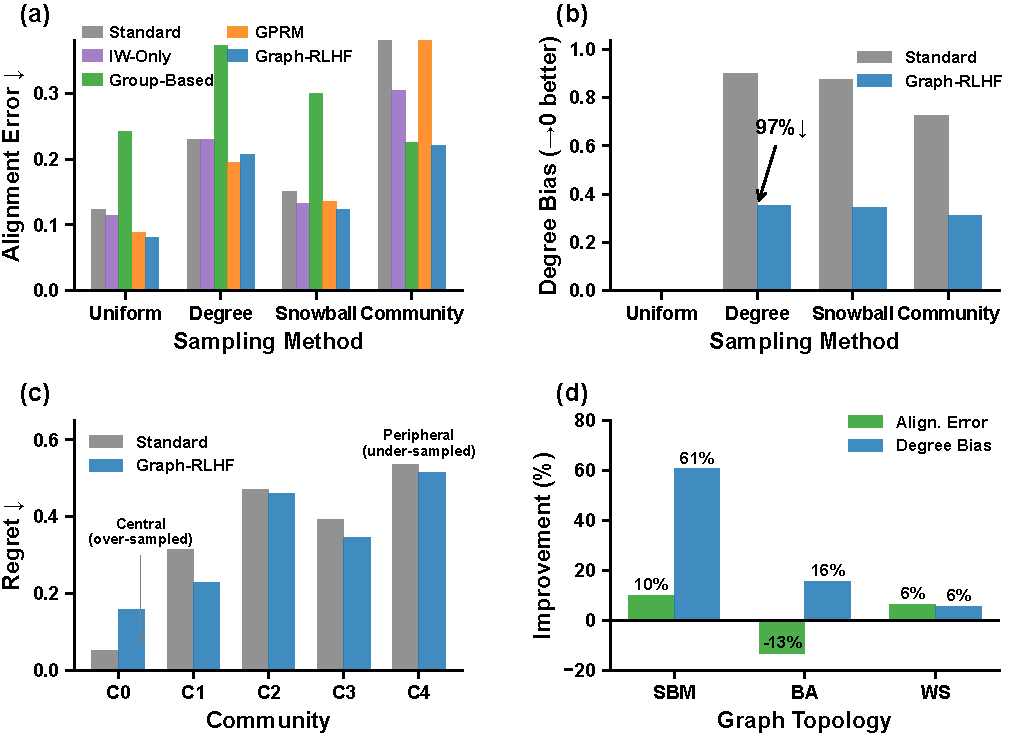
\includegraphics[width=\columnwidth]{figures/figure_main.pdf}
    \caption{Synthetic experiment analysis on SBM graph: (a)~Alignment error across sampling methods---Graph-RLHF achieves the lowest error under most bias patterns; (b)~Degree bias correction---our method effectively reduces the degree-weighted skew (97\% reduction); (c)~Per-community regret analysis under degree-biased sampling; (d)~Cross-graph generalization---consistent improvements on SBM (29\%), WS (18\%), and BA (7\%).}
    \label{fig:synthetic-results}
\end{figure}

% Cross-Graph Topology Comparison
\begin{table}[ht]
\caption{Cross-graph topology comparison under degree-biased sampling. \colorbox{bestgreen}{Green} = best, \colorbox{goodblue}{Blue} = our method.}
\label{tab:cross-graph}
\centering
\small
\begin{tabular}{llccc}
\toprule
\textbf{Graph} & \textbf{Method} & \textbf{Align.\ Err.}$\downarrow$ & \textbf{Deg.\ Bias}$\downarrow$ & \textbf{Improv.} \\
\midrule
\multirow{3}{*}{SBM}
& \cellcolor{neutralgray}Standard & \cellcolor{neutralgray}0.262{\tiny$\pm$0.08} & \cellcolor{neutralgray}0.062 & \cellcolor{neutralgray}--- \\
& GPRM (No GBA) & 0.245{\tiny$\pm$0.06} & 0.071 & 6\% \\
& \cellcolor{goodblue}\textbf{Graph-RLHF} & \cellcolor{bestgreen}\textbf{0.186}{\tiny$\pm$0.05} & \cellcolor{bestgreen}\textbf{0.002} & \cellcolor{bestgreen}\textbf{29\%} \\
\midrule
\multirow{3}{*}{BA}
& \cellcolor{neutralgray}Standard & \cellcolor{neutralgray}0.149{\tiny$\pm$0.02} & \cellcolor{neutralgray}0.005 & \cellcolor{neutralgray}--- \\
& GPRM (No GBA) & 0.131{\tiny$\pm$0.02} & 0.003 & 12\% \\
& \cellcolor{goodblue}\textbf{Graph-RLHF} & \cellcolor{bestgreen}\textbf{0.139}{\tiny$\pm$0.08} & \cellcolor{bestgreen}\textbf{0.000} & \cellcolor{goodblue}7\% \\
\midrule
\multirow{3}{*}{WS}
& \cellcolor{neutralgray}Standard & \cellcolor{neutralgray}0.123{\tiny$\pm$0.04} & \cellcolor{neutralgray}$-$0.000 & \cellcolor{neutralgray}--- \\
& GPRM (No GBA) & 0.125{\tiny$\pm$0.04} & $-$0.001 & $-$2\% \\
& \cellcolor{goodblue}\textbf{Graph-RLHF} & \cellcolor{bestgreen}\textbf{0.101}{\tiny$\pm$0.06} & \cellcolor{bestgreen}\textbf{0.000} & \cellcolor{bestgreen}\textbf{18\%} \\
\bottomrule
\end{tabular}
\end{table}

\section{Conclusion and Limitations}

We introduced Graph-RLHF, a framework that models annotators as nodes in a graph and corrects for network-induced sampling bias in RLHF. Our approach combines graph-personalized reward modeling with importance-weighted aggregation, providing theoretical guarantees on welfare deviation.

\paragraph{Limitations.}
(1) We assume the annotator graph is known or can be estimated; in practice, graph construction requires domain expertise.
(2) Our theoretical analysis focuses on population-level objectives; full finite-sample analysis of end-to-end policy optimization remains open.
(3) While we validate on the CA-1 dataset, further evaluation on diverse real-world RLHF deployments would strengthen generalizability claims.

% In the unusual situation where you want a paper to appear in the
% references without citing it in the main text, use \nocite
\nocite{langley00}

\bibliography{example_paper}
\bibliographystyle{icml2026}

%%%%%%%%%%%%%%%%%%%%%%%%%%%%%%%%%%%%%%%%%%%%%%%%%%%%%%%%%%%%%%%%%%%%%%%%%%%%%%%
%%%%%%%%%%%%%%%%%%%%%%%%%%%%%%%%%%%%%%%%%%%%%%%%%%%%%%%%%%%%%%%%%%%%%%%%%%%%%%%
% APPENDIX
%%%%%%%%%%%%%%%%%%%%%%%%%%%%%%%%%%%%%%%%%%%%%%%%%%%%%%%%%%%%%%%%%%%%%%%%%%%%%%%
%%%%%%%%%%%%%%%%%%%%%%%%%%%%%%%%%%%%%%%%%%%%%%%%%%%%%%%%%%%%%%%%%%%%%%%%%%%%%%%
\newpage
\appendix
\onecolumn

\section{Related Work}
\label{sec:related}

We review work on RLHF and alignment (Section~\ref{sec:rw_rlhf}), heterogeneous and personalized preferences (Section~\ref{sec:rw_personalized}), fairness and social choice in reward modeling (Section~\ref{sec:rw_fairness}), structured and graph-based feedback (Section~\ref{sec:rw_graph_feedback}), social network sampling and graph fairness (Section~\ref{sec:rw_network_bias}), and LLM-based simulations of human populations (Section~\ref{sec:rw_simulation}).
Throughout, we highlight that prior work treats human raters as an i.i.d.\ population or coarse groups, whereas we explicitly model them as nodes in a graph and correct for network-induced sampling bias.

\subsection{RLHF and Alignment}
\label{sec:rw_rlhf}

Modern RLHF pipelines emerged from the InstructGPT work of \citet{ouyang2022instructgpt}, which popularized the three-stage recipe of supervised fine-tuning, reward modeling from pairwise comparisons, and reinforcement learning to optimize the policy against the learned reward.
Subsequent work such as Direct Preference Optimization (DPO)~\citep{rafailov2023dpo} showed that one can bypass explicit reinforcement learning and directly optimize the policy against preferences, while RLAIF~\citep{lee2024rlaif} demonstrated that AI-generated feedback can partially substitute for human labels to scale alignment.
Recent surveys and monographs~\citep{kaufmann2025survey,lambert2025rlhfbook,shen2023llmalignment} synthesize this literature, covering reward modeling choices, optimization methods, and open challenges in aligning large language models.

These foundations treat human raters as an unstructured pool: annotations are modeled as i.i.d.\ draws from an abstract population, sometimes with per-rater reliability or noise parameters, but without any relational structure.
The PRISM alignment dataset~\citep{kirk2024prism} takes a major step toward richer feedback by collecting participatory, representative, and individualized responses from over 1{,}500 participants across 75 countries, making explicit the subjectivity and cultural diversity of alignment.
More recently, OpenAI's Collective Alignment dataset~\citep{openai2025ca1} collects value-sensitive preference data from over 1{,}000 globally distributed annotators with rich demographic information, revealing significant geographic imbalance in recruitment (36\% from the US alone).
However, even these datasets model participants as a set of individuals with attributes rather than as nodes in a network; their social or institutional ties and resulting sampling patterns are not represented.
In contrast, we treat annotators as vertices in a graph and ask how network structure itself shapes the reward signal that RLHF learns.

\subsection{Heterogeneous and Personalized Preferences}
\label{sec:rw_personalized}

A growing line of work studies RLHF under heterogeneous preferences.
\citet{poddar2024vpl} propose variational preference learning, modeling each rater with a latent preference vector so that the model can capture diverse tastes.
Personalized RLHF frameworks~\citep{li2024personalized_rlhf} formalize the problem of learning a personalized policy conditioned on user identity, and show that naive global RLHF can perform poorly for minority or atypical users.
Parameter-efficient approaches such as shared low-rank adaptations for personalized RLHF~\citep{liu2025shared_lora_prlhf} and reward factorization~\citep{shenfeld2025reward_factorization} decompose preferences into shared and user-specific components, enabling scalable personalization on top of a base model.
A recent survey on personalized alignment~\citep{guan2025personalized_alignment_survey} consolidates these methods and argues that personalization is a missing piece of human-aligned LLMs.

These works acknowledge that “one reward does not fit all” and that per-user conditioning can improve alignment.
However, users are still modeled as independent points in a feature space: there is no explicit notion of a social, institutional, or spatial graph connecting them.
In particular, they do not address how feedback is collected over networks (e.g., via platforms or peer recruitment), nor how network structure affects which preferences are over-represented.
Our work is complementary: we also allow preferences to vary between annotators, but we explicitly embed annotators in a graph and use this structure to regularize per-annotator utilities and to correct for network-induced sampling bias.

\subsection{Fairness, Group Robustness, and Social Choice in RLHF}
\label{sec:rw_fairness}

Several recent papers consider fairness and robustness across groups in RLHF.
MaxMin-RLHF~\citep{chakraborty2024maxminrlhf} formulates alignment as a minimax optimization over demographic or preference groups, maximizing the worst-group reward to avoid catastrophic under-alignment.
Group Robust Preference Optimization (GRPO)~\citep{ramesh2024grpo} studies robust preference optimization without explicit reward models, focusing on worst-group regret.
\citet{li2024optimizing_fair_stable} propose fair and stable composition of multiple reward signals in reinforcement learning for language models, controlling disparities and instability between reward components.
\citet{ouyang2025rewardfairness} explicitly analyze reward fairness in RLHF from a resource-allocation perspective, framing the allocation of reward mass across groups as a fairness problem.
Complementary benchmarks such as \citet{song2025groupfair_rewardmodels} systematically evaluate group fairness in reward models, revealing disparities across demographic groups even when average performance is high.
Work on fairness-aware reward optimization, such as FARO~\citep{choi2025faro}, further develops constrained objectives and certificates for reward fairness.

Parallel work brings tools from social choice theory into RLHF.
\citet{ge2024axioms} develop axioms for AI alignment from human feedback and show that standard Bradley--Terry models can violate natural social-choice properties, proposing linear social choice rules over pairwise comparisons.
\citet{dai2024mapping} map classic voting rules and impossibility results to RLHF, highlighting how contextual preferences and query selection differ from static elections.
\citet{conitzer2024socialchoice} argue that social choice should guide AI alignment when dealing with diverse human feedback, advocating for pluralistic alignment objectives and careful choice of welfare functions.
More recently, \citet{halpern2025pairwise_calibrated} introduce pairwise calibrated rewards for pluralistic alignment, designing reward models that better represent multiple value systems simultaneously.
From a statistical perspective, \citet{dumoulin2024density_pairwise} interpret learning from pairwise preferences as density estimation over latent utilities and highlight the misspecification that arises when a single reward is forced to represent heterogeneous annotators.

Taken together, this literature provides both normative desiderata (via social choice) and algorithmic tools (fairness-constrained and group-robust objectives) for aggregating diverse preferences.
However, the population of annotators is still treated as an i.i.d.\ set or partitioned into coarse groups.
The structure of interactions among annotators---who is connected, who is central, who influences whom---is absent from the models.
Our work extends this agenda by showing that even given a fixed social-welfare target (e.g., equal-per-person or equal-per-community), network-induced sampling can cause RLHF to optimize a very different, degree-weighted objective unless we explicitly correct for it.

\subsection{Structured and Graph-Based Feedback}
\label{sec:rw_graph_feedback}

Beyond human ratings, structured feedback sources are increasingly used in alignment.
RLKGF~\citep{yan2025rlkgf} proposes reinforcement learning from knowledge-graph feedback, using paths and relations in a knowledge graph as a signal for reward modeling, rather than human annotations.
This demonstrates that graph structure can be integrated into RLHF-style pipelines, and that rewards can be derived from structured, relational data.
However, in RLKGF the graph nodes are entities and relations in a domain, not human raters.
Similarly, RLAIF~\citep{lee2024rlaif} replaces some human preferences with feedback from an auxiliary model, but still treats feedback providers as an unstructured set.

Our setting is different: we focus on graphs of annotators, not graphs of entities or prompts.
The primary role of graph structure in our work is to capture how preferences cluster and how feedback is collected and propagated across a social or institutional network.
In that sense, we are closer in spirit to graph-aware fairness and sampling work (Section~\ref{sec:rw_network_bias}) than to knowledge-graph-based reward shaping.

\subsection{Social Network Sampling and Fairness on Graphs}
\label{sec:rw_network_bias}

Social network analysis and graph learning provide rich evidence that network structure profoundly shapes sampling, perception, and fairness.
Respondent-driven sampling (RDS) and related methods show that recruiting participants via their social ties leads to biased inclusion probabilities, typically over-sampling high-degree and well-connected individuals; inverse-probability weighting is necessary to obtain unbiased population estimates~\citep{wejnert2010rds}.
The ``majority illusion'' of \citet{lerman2016majorityillusion} demonstrates that behaviors that are globally rare can appear common in local neighborhoods because high-degree nodes disproportionately influence neighbors’ perceptions.
\citet{antunes2024minorityranking} analyze minority representation and ranking under sampling in attributed networks, showing that degree- and centrality-based sampling can distort the apparent prominence of minority groups.

In graph machine learning, structural and attribute bias have been documented and mitigated.
EDITS~\citep{dong2021edits} introduces a model-agnostic framework to debias graphs for GNNs, addressing both attribute and structural bias.
FairSNA~\citep{saxena2024fairsna} surveys algorithmic fairness in social network analysis, covering centrality, influence maximization, and community detection, and emphasizing how biased network structure leads to unfair outcomes.
Surveys on fairness-aware GNNs~\citep{chen2023fairgnn_survey} and fairness for machine learning on graphs~\citep{laclau2024fairness_graphs_survey} catalog a variety of fairness notions and mitigation strategies for node classification, link prediction, and other graph tasks.
Methods such as fairGNN-WOD~\citep{wang2025fairgnn_wod} tackle fair graph learning without complete demographic information by leveraging latent structure.

These works collectively argue that graphs are not neutral: who is connected to whom, and who is structurally central or peripheral, critically shapes both observations and downstream model behavior.
Yet, RLHF pipelines to date largely ignore these ideas and treat the set of annotators as if it were sampled uniformly at random from a population.
Our work brings insights from network sampling and fair graph learning into RLHF, modeling the rater graph explicitly and using it both to regularize per-annotator rewards and to debias aggregation toward a chosen social welfare target.

\subsection{LLM-Based Simulations and Networked Alignment}
\label{sec:rw_simulation}

Recent work uses LLMs themselves to simulate human populations and social processes.
\citet{aher2023turingexperiments} show that large language models can simulate multiple human participants and replicate classic human-subject experiments, introducing Turing-style experiments as a methodology for prototyping behavioral studies.
\citet{liu2023socially_aligned} train socially aligned language models on simulated social interactions between LLM agents, using multi-agent dialogues to learn social norms and behaviors.
A broader survey by \citet{gao2024llm_abm_survey} reviews agent-based modeling and simulation with LLM agents, including simulations of social networks, opinion dynamics, and institutional processes.

These works suggest that LLM-based simulations can approximate aspects of human behavior and social structure, and they motivate our use of simulated populations for lightweight experiments.
However, the focus is typically on phenomena within the simulated society (e.g., emergent norms), rather than on the sampling and aggregation of human feedback used to train another model.
Our framework is complementary: we model how feedback from humans embedded in a network is sampled and aggregated into a reward for RLHF, and we can use LLM-based agents on graphs as a testbed for studying these mechanisms without expensive human studies.

\subsection{Summary}

In summary, prior work on RLHF and alignment has developed powerful pipelines for learning from human preferences~\citep{ouyang2022instructgpt,rafailov2023dpo,kaufmann2025survey,lambert2025rlhfbook,shen2023llmalignment}, extended them to heterogeneous and personalized settings~\citep{poddar2024vpl,li2024personalized_rlhf,liu2025shared_lora_prlhf,shenfeld2025reward_factorization,guan2025personalized_alignment_survey}, and begun to incorporate fairness and social choice considerations in reward modeling~\citep{chakraborty2024maxminrlhf,ramesh2024grpo,li2024optimizing_fair_stable,ouyang2025rewardfairness,song2025groupfair_rewardmodels,choi2025faro,ge2024axioms,dai2024mapping,conitzer2024socialchoice,halpern2025pairwise_calibrated,dumoulin2024density_pairwise}.
In parallel, social network analysis and fair graph learning have shown that network structure induces sampling bias, perception distortions, and unfair outcomes~\citep{wejnert2010rds,lerman2016majorityillusion,antunes2024minorityranking,dong2021edits,saxena2024fairsna,chen2023fairgnn_survey,laclau2024fairness_graphs_survey,wang2025fairgnn_wod}.
Yet, RLHF methods largely ignore the annotator graph and assume i.i.d.\ feedback.
Our work is, to our knowledge, the first to formalize RLHF with networked annotators, to characterize the degree-weighted bias induced by graph-based sampling, and to propose a graph-aware reward modeling and aggregation framework that explicitly corrects for this bias while remaining compatible with existing RLHF and DPO pipelines.

%%%%%%%%%%%%%%%%%%%%%%%%%%%%%%%%%%%%%%%%%%%%%%%%%%%%%%%%%%%%%%%%%%%%%%%%%%%%%%%
%%%%%%%%%%%%%%%%%%%%%%%%%%%%%%%%%%%%%%%%%%%%%%%%%%%%%%%%%%%%%%%%%%%%%%%%%%%%%%%
\section{Additional Details for Problem Formulation}
\label{app:problem-details}

\subsection{Community Welfare and Disparity}
\label{app:community-welfare}

Let $\{C_k\}_{k=1}^K$ be a partition of $V$ into communities (e.g., detected via graph clustering). We define community-level welfare under a policy $\pi_\phi$ as
\begin{equation}
    W_k(\pi_\phi)
    =
    \frac{1}{|C_k|}
    \sum_{i \in C_k} U_i(\pi_\phi),
    \qquad
    k = 1,\dots,K.
    \label{eq:community-welfare}
\end{equation}
We measure community-level disparity via the max--min gap $\max_k W_k(\pi_\phi) - \min_k W_k(\pi_\phi)$, or alternatively the variance $\mathrm{Var}_k[W_k(\pi_\phi)]$. When $q_i \propto d_i$ (degree-proportional sampling), communities with higher average degree contribute disproportionately to the learned reward, potentially causing large welfare gaps across communities.

\subsection{Network-Based Sampling and Inclusion Probabilities}
\label{app:network-bias}

In many practical data-collection pipelines, annotators are recruited or
exposed to feedback interfaces through mechanisms that can be approximated by
network-based sampling. Two canonical examples are:

\begin{itemize}
    \item \textbf{Random walks on $G$.} Suppose at each step we select a node
    $i$ and then move to a random neighbor $j \in N(i)$, and solicit feedback
    from the current node. Under mild conditions, the stationary distribution
    of this Markov chain is proportional to node degree:
    $q_i \propto d_i$.
    \item \textbf{Respondent-driven sampling.} In respondent-driven sampling
    (RDS), initial ``seed'' participants recruit neighbors (e.g., friends or
    colleagues), who in turn recruit further participants. The resulting
    sample is known to over-represent high-degree nodes; estimators of the
    inclusion probabilities $q_i$ often take the form $q_i \propto d_i$ or
    functions thereof.
\end{itemize}

These mechanisms are not meant to be exact models of how RLHF data is
collected, but they capture the qualitative fact that annotators with larger
degree or centrality in $G$ tend to have higher $q_i$. Our method does not
require knowing the exact sampling mechanism; Section~\ref{sec:method} works
with any estimator $\hat q_i$ of the inclusion probabilities.

\subsection{Consistency of Scalar Reward Modeling under the Population Model}
\label{app:consistency}

For completeness, we sketch why standard scalar reward modeling recovers the
$q$-weighted social welfare under Assumption~\ref{ass:scalar-q}.

Under Assumption~\ref{ass:scalar-q}, there exists a scalar reward
$r_q^\star(x,y)$ such that the probability that a randomly observed
preference pair satisfies $y^+ \succ y^-$ is
\begin{equation}
    \Pr(y^+ \succ y^- \mid x)
    =
    \sigma\!\big(r_q^\star(x,y^+) - r_q^\star(x,y^-)\big).
\end{equation}

When individual preferences follow a logistic model
$\Pr(y^+ \succ y^- \mid x, i) = \sigma(u_i(x,y^+) - u_i(x,y^-))$, the marginal
is a mixture:
$\Pr(y^+ \succ y^- \mid x) = \sum_i q_i \sigma(\Delta u_i)$.
If individual utilities are not too dispersed, this mixture is
well-approximated by a single logistic model with logit
\begin{equation}
    \ell(x, y^+, y^-)
    \approx
    \sum_{i \in V} q_i \,
    \left( u_i(x,y^+) - u_i(x,y^-) \right),
\end{equation}
and $r_q^\star(x,y) \propto \sum_i q_i u_i(x,y)$.

Training a scalar reward model $r_\theta(x,y)$ by maximum-likelihood with the
standard Bradley--Terry loss,
\begin{equation}
    \mathcal{L}_{\text{BTL}}(\theta)
    =
    - \sum_{t=1}^T
    \log \sigma\!\left( r_\theta(x_t, y_t^+) - r_\theta(x_t, y_t^-) \right),
\end{equation}
yields a consistent estimator of $r_q^\star$ as $T \to \infty$ under standard
regularity conditions. Consequently, the induced policy optimization step in
RLHF is effectively maximizing the $q$-weighted social welfare
\begin{equation}
    W_{\text{obs}}(\pi_\phi)
    =
    \sum_{i \in V} q_i \, U_i(\pi_\phi),
\end{equation}
not the target welfare $W_{\text{target}}$ in
Definition~\ref{def:target-welfare}. This mismatch is precisely the
network-induced misalignment quantified in \eqref{eq:misalignment}.

%%%%%%%%%%%%%%%%%%%%%%%%%%%%%%%%%%%%%%%%%%%%%%%%%%%%%%%%%%%%%%%%%%%%%%%%%%%%%%%
%%%%%%%%%%%%%%%%%%%%%%%%%%%%%%%%%%%%%%%%%%%%%%%%%%%%%%%%%%%%%%%%%%%%%%%%%%%%%%%
\section{Additional Details for Method}
\label{app:method-details}

\subsection{Solving the Graph-Balanced Weight Optimization}
\label{app:wstar-details}

Recall the optimization problem for the importance weights $\alpha^\star$:
\begin{equation}
\begin{aligned}
    \min_{\alpha \in \mathbb{R}^{|V|}}
    \quad &
    \frac{1}{2} \|\alpha - \tilde\alpha\|_2^2
    + \lambda_{\text{smooth}} \, \alpha^\top L_w \alpha
    + \lambda_{\text{comm}} \sum_{k=1}^{K}
      \Big( \sum_{i \in C_k} \hat q_i \alpha_i - \rho_k \Big)^2
    + \lambda_{\text{var}} \sum_{i \in V} \hat q_i \alpha_i^2
    \\
    \text{s.t.}\quad
    & \alpha_i \ge 0 \ \forall i \in V,
    \quad
    \sum_{i \in V} \hat q_i \alpha_i = 1,
\end{aligned}
\label{eq:alpha-star-appendix}
\end{equation}
where $\tilde\alpha_i = \pi_i / (\hat q_i + \varepsilon)$ as defined in
\eqref{eq:alpha-raw}, $L_w$ is the weighted graph Laplacian, $\lambda_{\text{smooth}} \ge 0$
controls graph smoothness, $\lambda_{\text{comm}} \ge 0$ controls community
balance, $\lambda_{\text{var}} \ge 0$ controls variance (and hence ESS),
and $\rho_k$ are the target community masses in the induced distribution
(e.g., $\rho_k = 1/K$ for equal-per-community welfare).

Problem~\eqref{eq:alpha-star-appendix} is a convex quadratic program (QP).
In our experiments, we solve it using a projected gradient method:

\begin{enumerate}
    \item Initialize $\alpha^{(0)} = \tilde\alpha$, then project onto
    the feasible set $\{\alpha \ge 0, \sum_i \hat q_i \alpha_i = 1\}$.
    \item At iteration $s$, compute the gradient. Let
    $A_k(\alpha) = \sum_{i \in C_k} \hat q_i \alpha_i$ denote the induced
    community-$k$ mass. Then
    \begin{equation}
        \nabla f(\alpha^{(s)})_i
        = \alpha_i^{(s)} - \tilde\alpha_i
        + 2 \lambda_{\text{smooth}} (L_w \alpha^{(s)})_i
        + 2 \lambda_{\text{comm}} \hat q_i (A_{k(i)}(\alpha^{(s)}) - \rho_{k(i)})
        + 2 \lambda_{\text{var}} \hat q_i \alpha_i^{(s)},
    \end{equation}
    where $k(i)$ is the community containing annotator $i$.
    \item Take a gradient step
    $z^{(s+1)} = \alpha^{(s)} - \eta \nabla f(\alpha^{(s)})$ with step size
    $\eta$.
    \item Project $z^{(s+1)}$ onto the feasible set
    $\{\alpha \ge 0, \sum_i \hat q_i \alpha_i = 1\}$ using weighted simplex
    projection.
\end{enumerate}

The Laplacian term $\alpha^\top L_w \alpha$ can be computed efficiently using
sparse matrix--vector operations. In practice we find that a small number of
iterations (e.g., 50--100) suffices for convergence on graphs with up to tens
of thousands of annotators.

\begin{proposition}[Stability of $\alpha^\star$ under perturbations]
\label{prop:alpha-stability}
Let $J(\alpha)$ be the objective in \eqref{eq:alpha-star} (ignoring
constraints for clarity). Its Hessian is
\[
    H = I + 2\lambda_{\mathrm{smooth}} L_w
      + 2\lambda_{\mathrm{comm}} B^\top B
      + 2\lambda_{\mathrm{var}} \mathrm{diag}(\hat q),
\]
where $B$ encodes community-mass linear forms. Since $L_w \succeq 0$,
$B^\top B \succeq 0$, and
$\mathrm{diag}(\hat q) \succeq \hat q_{\min} I$, we have
$H \succeq \mu I$ with $\mu = 1 + 2\lambda_{\mathrm{var}} \hat q_{\min}$.
Therefore the unconstrained minimizer mapping is $(1/\mu)$-Lipschitz in
the gradient, and the constrained minimizer over a convex feasible set
remains nonexpansive under projection. In particular, small perturbations
in $(L_w, \hat q, \tilde\alpha)$ imply
$\|\alpha^\star - \alpha^{\star\prime}\|_2 \le
\frac{1}{\mu} \|\nabla J - \nabla J'\|_2$.
\end{proposition}

\subsection{Approximation to Target Welfare}
\label{app:welfare-approx}

We justify why using the induced welfare weights $\tilde\pi_i = \hat q_i \alpha_i^\star$
in the reward aggregation approximates optimizing the target welfare
$W_{\text{target}}(\pi_\phi)$.

Assume that:
(i) the personalized reward model $r_\theta(x,y,i)$ is a well-calibrated
estimator of the latent utility $u_i(x,y)$ (in the sense that
$r_\theta(x,y,i) \approx u_i(x,y)$ up to a global affine transformation),
and (ii) the importance weights $\alpha_i^\star$ solve the debiasing problem in
Section~\ref{subsec:gba}, so that the induced distribution
$\tilde\pi_i = \hat q_i \alpha_i^\star$ approximates $\pi_i$.

Given a policy $\pi_\phi$, the expected aggregated reward is
\begin{align}
    \mathbb{E}_{x,y}\!\left[ \bar r_\theta(x,y) \right]
    &= \mathbb{E}_{x \sim p_{\text{data}}, y \sim \pi_\phi(\cdot \mid x)}
    \left[ \sum_{i \in V} \tilde\pi_i \, r_\theta(x,y,i) \right] \nonumber
    \\
    &\approx
    \sum_{i \in V} \tilde\pi_i \,
    \mathbb{E}_{x,y} \left[ u_i(x,y) \right]
    =
    \sum_{i \in V} \tilde\pi_i \, U_i(\pi_\phi)
    =
    \widetilde{W}(\pi_\phi).
\end{align}
By Proposition~\ref{prop:welfare-gap}, the difference between
$\widetilde{W}(\pi_\phi)$ and $W_{\text{target}}(\pi_\phi)$ is bounded by
$R \|\pi - \tilde\pi\|_1$, where $R$ is the utility range. When
$\alpha_i^\star = \pi_i / q_i$ exactly (no smoothing or community constraints),
we have $\tilde\pi = \pi$ and the approximation is exact.

\subsection{Reward-Model-Based Graph-RLHF (PPO Variant)}
\label{app:ppo}

Instead of using Graph-DPO, we can leverage the aggregated reward
$\bar r_\theta(x,y)$ directly in a reward-model-based RLHF setup. We outline
a PPO variant here.

At training time, the policy $\pi_\phi$ interacts with an environment (or
generates trajectories from a dataset of prompts) to produce sequences
$\tau = (x_1, y_1, \dots, x_T, y_T)$. For each time step $t$, we compute a
scalar reward
\begin{equation}
    R_t = \bar r_\theta(x_t, y_t),
\end{equation}
where $\bar r_\theta$ is defined in \eqref{eq:aggregated-reward}. We then
compute advantages $A_t$ using a standard value-function baseline and optimize
the PPO objective
\begin{equation}
    \mathcal{L}_{\text{PPO}}(\phi)
    =
    - \mathbb{E}_t
    \left[
    \min\Big(
        r_t(\phi) A_t,\,
        \text{clip}\big(r_t(\phi), 1 - \epsilon, 1 + \epsilon\big) A_t
    \Big)
    \right],
\end{equation}
where $r_t(\phi) = \pi_\phi(y_t \mid x_t) / \pi_{\phi_{\text{old}}}(y_t \mid x_t)$
and $\epsilon$ is the clipping parameter.

Because $\bar r_\theta$ incorporates the induced welfare weights
$\tilde\pi_i = \hat q_i \alpha_i^\star$, the resulting policy is encouraged
to maximize the induced welfare $\widetilde{W}(\pi_\phi)$ rather than the
observed welfare $W_{\text{obs}}(\pi_\phi)$ that would be induced by a
reward model trained without importance weighting. When importance weights
achieve exact debiasing ($\alpha_i^\star = \pi_i / q_i$), the induced welfare
equals the target welfare.

\subsection{Graph-Active Feedback Algorithm}
\label{app:active}

Algorithm~\ref{alg:graph-active} summarizes one possible instantiation of the
graph-active feedback strategy mentioned in Section~\ref{sec:method}.

\begin{algorithm}[h]
    \caption{Graph-Active Feedback Selection}
    \label{alg:graph-active}
    \begin{algorithmic}[1]
        \REQUIRE Annotator graph $G=(V,E)$, target weights $\pi_i$, current
        induced weights $\tilde\pi_i = \hat q_i \alpha_i$, personalized
        rewards $r_\theta$, budget $B$.
        \STATE Sample a batch of prompts $\{x_s\}_{s=1}^S$ and candidate
        outputs.
        \FOR{each annotator $i \in V$}
            \STATE Compute a disagreement score
            \[
                \text{disc}(i)
                =
                \frac{1}{S}
                \sum_{s=1}^S
                \left|
                    r_\theta(x_s, y_s^\star, i)
                    -
                    \bar r_\theta(x_s, y_s^\star)
                \right|,
            \]
            where $y_s^\star$ is a reference output (e.g., sampled from the
            current policy).
            \STATE Compute an under-representation score
            $\text{repr}(i) = \pi_i / (\tilde\pi_i + \epsilon)$.
            \STATE Set
            $a(i) =
            \alpha_{\mathrm{disc}} \cdot \text{disc}(i)
            +
            \alpha_{\mathrm{repr}} \cdot \text{repr}(i)$.
        \ENDFOR
        \STATE Select a batch $S \subset V$ of size $B$ by greedily adding
        the node with largest $a(i)$ minus a redundancy penalty for neighbors
        already in $S$:
        \[
            i^\star
            =
            \arg\max_{i \in V \setminus S}
            \Big(
                a(i)
                -
                \alpha_{\mathrm{red}} \sum_{j \in S} \mathbb{I}\{(i,j) \in E\}
            \Big).
        \]
        \STATE Query annotators in $S$ for new preference labels and update
        the GPRM and importance weights $\alpha_i$ (hence
        $\tilde\pi_i = \hat q_i \alpha_i$).
    \end{algorithmic}
\end{algorithm}

The redundancy penalty discourages selecting annotators that are immediate
neighbors of each other, encouraging coverage of diverse regions of the
graph. The hyperparameters
$\alpha_{\mathrm{disc}}, \alpha_{\mathrm{repr}}, \alpha_{\mathrm{red}}$
control the trade-off between disagreement, under-representation, and
exploration of the graph.


\section{Additional Theoretical Details}
\label{app:theory-details}

% --- DROP-IN: new appendix proof for mixture bound ---
\subsection{Mixture-of-Logits Approximation Bound}
\label{app:proof-mixture}

This section provides the formal bound mentioned in Section~\ref{sec:problem}. Suppose individual preferences follow a logistic model
$\Pr(y^+ \succ y^- \mid x,i)=\sigma(\Delta u_i)$ where 
$\Delta u_i := u_i(x,y^+) - u_i(x,y^-)$.
The marginal preference probability is a mixture of logits:
$\Pr(y^+ \succ y^- \mid x)=\sum_{i \in V} q_i \sigma(\Delta u_i)$.
Let $m := \mathbb{E}_{i\sim q}[\Delta u_i]$ and let 
$\mathrm{range}(\Delta u):=\max_i \Delta u_i-\min_i \Delta u_i$.
Using that $\sigma$ is $1/4$-Lipschitz, we have the approximation bound
\begin{equation}
\Big|
\mathbb{E}_{i\sim q}[\sigma(\Delta u_i)]-\sigma(m)
\Big|
\;\le\;
\frac{1}{4}\,\mathbb{E}_{i\sim q}\big|\Delta u_i-m\big|
\;\le\;
\frac{1}{8}\,\mathrm{range}(\Delta u).
\label{eq:mixture-bound}
\end{equation}
Thus when preference heterogeneity is small on a given comparison, a scalar
logit $\sigma(m)$ approximates the mixture well.

\begin{proof}
Let $X$ be the random variable $X=\Delta u_i$ when $i\sim q$, and let
$m=\mathbb{E}[X]$. Since the derivative of the sigmoid satisfies
$\sup_z \sigma'(z)=1/4$, the function $\sigma(\cdot)$ is $1/4$-Lipschitz:
$|\sigma(a)-\sigma(b)|\le \frac{1}{4}|a-b|$ for all $a,b\in\mathbb{R}$.
Therefore,
\[
\Big|\mathbb{E}[\sigma(X)]-\sigma(m)\Big|
=
\Big|\mathbb{E}[\sigma(X)]-\mathbb{E}[\sigma(m)]\Big|
\le 
\mathbb{E}\big[|\sigma(X)-\sigma(m)|\big]
\le
\frac{1}{4}\,\mathbb{E}[|X-m|].
\]
For the second inequality in Eq.~\eqref{eq:mixture-bound}, note that $X$ is
supported on the interval $[\min_i \Delta u_i,\max_i \Delta u_i]$ and the mean
$m$ lies in the same interval. A standard extremal argument for bounded random
variables gives $\mathbb{E}|X-m|\le \frac{1}{2}(\max_i \Delta u_i-\min_i \Delta u_i)$,
yielding $\mathbb{E}|X-m|\le \frac{1}{2}\mathrm{range}(\Delta u)$ and hence
Eq.~\eqref{eq:mixture-bound}.
\end{proof}

% --- DROP-IN B: new appendix proof section for split theorem/corollary ---
\subsection{Proofs for Theorem~\ref{thm:naive-q-objective} and Corollary~\ref{cor:naive-q-weighted-welfare}}
\label{app:proof-naive-split}

\subsubsection{Proof of Theorem~\ref{thm:naive-q-objective}}
\begin{proof}
Let $(I,X,Y^+,Y^-)$ be drawn by first sampling $I\sim q$ over $V$ and then
$(X,Y^+,Y^-)\sim \mathcal{T}(I)$. By the law of total expectation,
\[
\mathcal{L}_{\text{naive}}(\theta)
=
\mathbb{E}\big[\ell_{\text{naive}}(\theta;X,Y^+,Y^-)\big]
=
\sum_{i\in V}\Pr(I=i)\,
\mathbb{E}\big[\ell_{\text{naive}}(\theta;X,Y^+,Y^-)\mid I=i\big],
\]
which is exactly \eqref{eq:naive-q-mixture-risk}, with
$\mathcal{L}_i(\theta)=\mathbb{E}_{(x,y^+,y^-)\sim\mathcal{T}(i)}[\ell_{\text{naive}}(\theta;x,y^+,y^-)]$.

For the gradient identity, assume $\nabla_\theta \ell_{\text{naive}}(\theta;\cdot)$
is dominated by an integrable function in a neighborhood of $\theta$ (or simply
bounded, which holds if rewards are clipped / regularized and the dataset support is bounded).
Then differentiation under the integral is valid, yielding
\[
\nabla_\theta \mathcal{L}_{\text{naive}}(\theta)
=
\nabla_\theta \sum_{i\in V} q_i \mathcal{L}_i(\theta)
=
\sum_{i\in V} q_i \nabla_\theta \mathcal{L}_i(\theta),
\]
which is \eqref{eq:naive-q-mixture-grad}.
\end{proof}

\subsubsection{Proof of Corollary~\ref{cor:naive-q-weighted-welfare}}
\begin{proof}
\textbf{Step 1 (consistency of naive reward modeling).}
Under Assumption~\ref{ass:well-specified}, there exists a scalar reward function
$r^\star$ such that for all $(x,y^+,y^-)$,
\[
\Pr(y^+ \succ y^- \mid x)
=
\sigma\big(r^\star(x,y^+)-r^\star(x,y^-)\big),
\]
where the probability is with respect to the marginal data-generating process
(induced by sampling $i\sim q$ and then $(x,y^+,y^-)\sim\mathcal{T}(i)$).
Training $r_\theta(x,y)$ by maximum likelihood with Bradley--Terry loss is
equivalent to logistic regression on pairwise differences, and the negative
log-likelihood is minimized (over a rich enough function class) when the model
probabilities match the true conditional probabilities. Since the sigmoid link is
strictly monotone, this identifies $r^\star$ up to an additive constant. Thus,
with sufficient data and capacity, naive reward modeling recovers $r^\star$ (up to a constant).

\textbf{Step 2 (reward maximization equals $q$-weighted welfare).}
Assumption~\ref{ass:welfare-consistent} states that there exist constants
$a > 0$ and $b \in \mathbb{R}$ such that
\[
r^\star(x,y) = a \sum_{i\in V} q_i u_i(x,y) + b.
\]
Therefore, for any policy $\pi_\phi$,
\[
\mathbb{E}_{x\sim p_{\mathrm{data}},\,y\sim\pi_\phi(\cdot\mid x)}[r^\star(x,y)]
=
a \, \mathbb{E}_{x,y}\left[\sum_{i\in V} q_i u_i(x,y)\right] + b
=
a \sum_{i\in V} q_i U_i(\pi_\phi) + b
=
a \, W_{\mathrm{obs}}(\pi_\phi) + b.
\]
Because $a > 0$ and $b$ is a constant independent of $\pi_\phi$, maximizing
the expected reward is equivalent to maximizing $W_{\mathrm{obs}}(\pi_\phi)$,
which proves the claim.
\end{proof}

\subsection{Proof of Lemma~\ref{lem:iw-identity}}
\label{app:proof-iw}

\begin{lemma*}[Importance-weighted objective equals induced mixture]
Let $i \sim q$ and let $\alpha$ be any nonnegative weights. Define the
induced distribution $\tilde\pi_i := q_i \alpha_i$ and suppose
$\sum_i \tilde\pi_i = 1$. Then for any per-annotator population quantity
$h_i(\theta)$,
\begin{equation}
    \sum_{i \in V} q_i \alpha_i \, h_i(\theta)
    =
    \sum_{i \in V} \tilde\pi_i \, h_i(\theta).
\end{equation}
In particular, when $\alpha_i = \pi_i / q_i$ (and $q_i > 0$), we have
$\tilde\pi = \pi$.
\end{lemma*}

\begin{proof}
The identity is immediate from the definition $\tilde\pi_i = q_i \alpha_i$:
\begin{equation}
    \sum_{i \in V} q_i \alpha_i \, h_i(\theta)
    =
    \sum_{i \in V} \tilde\pi_i \, h_i(\theta).
\end{equation}
For the second claim, when $\alpha_i = \pi_i / q_i$, we have
\begin{equation}
    \tilde\pi_i = q_i \cdot \frac{\pi_i}{q_i} = \pi_i,
\end{equation}
so $\tilde\pi = \pi$.

When using estimated inclusion probabilities $\hat q_i$, the induced
distribution becomes $\tilde\pi_i = \hat q_i \alpha_i$. Under
Assumption~\ref{ass:qhat}, $\hat q_i \to q_i$ as $T \to \infty$, so the
induced distribution converges to the idealized version $q_i \alpha_i$.
\end{proof}

\subsection{Proof of Theorem~\ref{thm:graph-welfare}}
\label{app:proof-graph-welfare}

\begin{theorem*}[Graph-RLHF optimizes the induced welfare]
Assume (i) $\hat q = q$ and $\alpha^\star$ is the solution of
\eqref{eq:alpha-star}, (ii) the personalized reward model satisfies
$r_{\theta^\star}(x,y,i) = a \, u_i(x,y) + b$ for $a > 0$ and $b$ independent
of $i$, and (iii) policy optimization maximizes
$\mathbb{E}_{x,y \sim \pi_\phi}[\bar r_{\theta^\star}(x,y)]$.
Then the resulting policy maximizes the induced welfare
$\widetilde{W}(\pi_\phi) = \sum_i \tilde\pi_i U_i(\pi_\phi)$, where
$\tilde\pi_i = q_i \alpha_i^\star$. Moreover, if
$\alpha_i^\star = \pi_i / q_i$ (exact debiasing), then
$\widetilde{W} = W_{\text{target}}$.
\end{theorem*}

\begin{proof}
\textbf{Part (1): Reward model recovery.}
By Lemma~\ref{lem:iw-identity}, the importance-weighted population loss
$\sum_i q_i \alpha_i \ell(\theta; i)$ equals $\sum_i \tilde\pi_i \ell(\theta; i)$,
the loss under the induced distribution $\tilde\pi = q \odot \alpha$.
Under Assumption~\ref{ass:expressive}, there exists $\theta^\star$ such that
$r_{\theta^\star}(x,y,i) = a \, u_i(x,y) + b$ for $a > 0$ and $b$ shared across
all annotators.
Because the Bradley--Terry loss is a strictly proper scoring rule for pairwise
preferences (see, e.g., \citealt{gneiting2007strictly}), the unique minimizer
recovers individual utilities up to a shared affine transformation.

\textbf{Part (2): Aggregated reward structure.}
By the definition of aggregated reward in Eq.~\eqref{eq:aggregated-reward},
\begin{equation}
    \bar r_{\theta^\star}(x,y)
    =
    \sum_{i \in V} \tilde\pi_i r_{\theta^\star}(x,y,i)
    =
    \sum_{i \in V} \tilde\pi_i \big(a \, u_i(x,y) + b\big)
    =
    a \sum_{i \in V} \tilde\pi_i u_i(x,y) + b,
\end{equation}
where we used $\sum_i \tilde\pi_i = 1$.

\textbf{Part (3): Policy optimization.}
For any policy $\pi_\phi$, the expected aggregated reward is
\begin{equation}
    \mathbb{E}_{x,y}[\bar r_{\theta^\star}(x,y)]
    =
    \sum_{i \in V} \tilde\pi_i \, \mathbb{E}_{x,y}[u_i(x,y)] + c
    =
    \sum_{i \in V} \tilde\pi_i U_i(\pi_\phi) + c
    =
    \widetilde{W}(\pi_\phi) + c.
\end{equation}
Because $c$ is independent of $\pi_\phi$, maximizing
$\mathbb{E}_{x,y}[\bar r_{\theta^\star}(x,y)]$ is equivalent to maximizing
$\widetilde{W}(\pi_\phi)$.

\textbf{Part (4): Exact debiasing.}
When $\alpha_i^\star = \pi_i / q_i$, we have
$\tilde\pi_i = q_i \cdot (\pi_i / q_i) = \pi_i$, so
$\widetilde{W}(\pi_\phi) = \sum_i \pi_i U_i(\pi_\phi) = W_{\text{target}}(\pi_\phi)$.
\end{proof}

\subsection{Proof of Proposition~\ref{prop:community-balance}}
\label{app:proof-community}

% --- DROP-IN: REPLACE proof in Appendix~\ref{app:proof-community} ---
\begin{proof}
Fix the feasible set
\[
\mathcal{F}:=\{\alpha\in\mathbb{R}^{|V|}:\ \alpha\ge 0,\ \sum_{i\in V}\hat q_i\alpha_i=1\}.
\]
Define the continuous function
\[
g(\alpha):=
\frac{1}{2}\|\alpha-\tilde\alpha\|_2^2
+\lambda_{\mathrm{smooth}}\alpha^\top L_w\alpha
+\lambda_{\mathrm{var}}\sum_i \hat q_i\alpha_i^2,
\]
and the community-mass deviations
$A_k(\alpha):=\sum_{i\in C_k}\hat q_i\alpha_i$.
Then the objective in Eq.~\eqref{eq:alpha-star} can be written as
\[
J_\lambda(\alpha)=g(\alpha)+\lambda\sum_{k=1}^K (A_k(\alpha)-\rho_k)^2,
\qquad \lambda=\lambda_{\mathrm{comm}}.
\]

\textbf{Step 1 (existence of an exactly balanced feasible point).}
Let $Q_k:=\sum_{i\in C_k}\hat q_i$ (note $Q_k>0$ if $\hat q_i>0$ on each community).
Define $\alpha^{(0)}$ by setting, for each $i\in C_k$,
\[
\alpha_i^{(0)}:=\frac{\rho_k}{Q_k}.
\]
Then $\alpha^{(0)}\ge 0$, and
$A_k(\alpha^{(0)})=\sum_{i\in C_k}\hat q_i(\rho_k/Q_k)=\rho_k$ for all $k$.
Also $\sum_i \hat q_i\alpha_i^{(0)}=\sum_k \rho_k=1$, so $\alpha^{(0)}\in\mathcal{F}$.

\textbf{Step 2 (boundedness and vanishing penalty).}
Let $\alpha^{(\lambda)}$ be the unique minimizer of $J_\lambda$ over $\mathcal{F}$
(uniqueness holds because $J_\lambda$ is strictly convex on $\mathcal{F}$ due to
the $\frac12\|\alpha-\tilde\alpha\|^2$ term).
By optimality,
\[
J_\lambda(\alpha^{(\lambda)}) \le J_\lambda(\alpha^{(0)}) = g(\alpha^{(0)}),
\]
since the penalty term vanishes at $\alpha^{(0)}$.
Therefore,
\[
\lambda\sum_{k=1}^K (A_k(\alpha^{(\lambda)})-\rho_k)^2
\le J_\lambda(\alpha^{(\lambda)}) \le g(\alpha^{(0)}),
\]
which implies
\[
\sum_{k=1}^K (A_k(\alpha^{(\lambda)})-\rho_k)^2 \le \frac{g(\alpha^{(0)})}{\lambda}
\;\xrightarrow[\lambda\to\infty]{}\; 0.
\]
Hence $A_k(\alpha^{(\lambda)})\to \rho_k$ for each $k=1,\dots,K$, proving the claim.
\end{proof}

\subsection{Proof of Proposition~\ref{prop:welfare-gap}}
\label{app:proof-welfare-gap}

\begin{proposition*}[Welfare deviation bound via weight mismatch]
Assume $|U_i(\pi_\phi)| \le R$ for all $i$ and policies $\pi_\phi$. Let
$\pi$ be the target weights and let $\tilde\pi$ be the induced weights
used by Graph-RLHF. Then for any policy $\pi_\phi$,
\begin{equation}
    \big|
        W_{\text{target}}(\pi_\phi)
        -
        \widetilde{W}(\pi_\phi)
    \big|
    \le
    R \, \|\pi - \tilde\pi\|_1.
\end{equation}
\end{proposition*}

\begin{proof}
By definition of the welfare functions,
\begin{equation}
    W_{\text{target}}(\pi_\phi) = \sum_{i \in V} \pi_i U_i(\pi_\phi),
    \qquad
    \widetilde{W}(\pi_\phi) = \sum_{i \in V} \tilde\pi_i U_i(\pi_\phi),
\end{equation}
where $\tilde\pi_i = \hat q_i \alpha_i^\star$ is the induced welfare weight.
The difference is
\begin{equation}
    W_{\text{target}}(\pi_\phi) - \widetilde{W}(\pi_\phi)
    =
    \sum_{i \in V} (\pi_i - \tilde\pi_i) U_i(\pi_\phi)
    =
    (\pi - \tilde\pi)^\top U(\pi_\phi).
\end{equation}
Applying the bound $|U_i(\pi_\phi)| \le R$ and the triangle inequality:
\begin{equation}
    \big|
        W_{\text{target}}(\pi_\phi) - \widetilde{W}(\pi_\phi)
    \big|
    \le
    \sum_{i \in V} |\pi_i - \tilde\pi_i| \cdot |U_i(\pi_\phi)|
    \le
    R \sum_{i \in V} |\pi_i - \tilde\pi_i|
    =
    R \, \|\pi - \tilde\pi\|_1,
\end{equation}
as claimed. This bound is tight in the sense that it can be achieved when
$U_i(\pi_\phi) = R \cdot \text{sign}(\pi_i - \tilde\pi_i)$ for all $i$.
\end{proof}

%%%%%%%%%%%%%%%%%%%%%%%%%%%%%%%%%%%%%%%%%%%%%%%%%%%%%%%%%%%%%%%%%%%%%%%%%%%%%%%
\section{Additional Experimental Details}
\label{app:exp-details}

\subsection{Synthetic Experiment Implementation}
\label{app:synthetic-impl}

\paragraph{Graph topologies.}
To ensure robustness across network structures, we generate three types of graphs ($N=500$):
\begin{itemize}
    \item \textbf{Stochastic Block Model (SBM):} $K=4$ communities with a hub-and-spoke structure. The hub community (40\% of nodes) has dense internal connections ($p=0.15$), while spoke communities (20\% each) are sparser ($p=0.08$). Inter-community probability is $p=0.01$.
    \item \textbf{Barabási-Albert (BA):} A scale-free network generated via preferential attachment with $m=5$ edges per new node. This models networks with extreme degree distributions (power-law).
    \item \textbf{Watts-Strogatz (WS):} A small-world network with $k=10$ nearest neighbors and rewiring probability $p=0.1$, exhibiting high clustering coefficients.
\end{itemize}

\paragraph{Utility functions and Heterophily.}
We model utilities as $u_i(x,y) = w_i^\top \phi(x,y)$, where $\phi(x,y) \in \mathbb{R}^{10}$. The weight vectors $w_i$ are generated with a hierarchical structure:
$w_i = w_{\text{shared}} + w_{c(i)}^{\text{comm}} + \epsilon_i$, where $\epsilon_i \sim \mathcal{N}(0, \sigma^2 I)$.
To test robustness against heterophily, we introduce a \texttt{heterophily\_ratio} parameter $\rho_h$. We randomly select $\rho_h \cdot N$ nodes and ``flip'' their community preference component ($w_{c(i)}^{\text{comm}} \leftarrow -w_{c(i)}^{\text{comm}}$), simulating adversarial users who disagree with their local community.

\paragraph{Sampling Mechanisms.}
We simulate four distinct feedback collection processes:
\begin{itemize}
    \item \textbf{Uniform:} $q_i = 1/N$.
    \item \textbf{Degree-Biased:} $q_i \propto \text{deg}(i)^\gamma$ (default $\gamma=1.5$).
    \item \textbf{Snowball:} A random walk-based process starting from $S$ seeds, naturally over-sampling high-centrality nodes.
    \item \textbf{Community-Biased:} Biased towards specific communities (e.g., Hub community has $5\times$ inclusion probability), simulating platform demographic bias.
\end{itemize}

\paragraph{Baselines.}
We compare Graph-RLHF against a comprehensive suite of baselines:
\begin{itemize}
    \item \textbf{Standard:} Naive scalar reward model trained on all data.
    \item \textbf{IW-only:} Standard model trained with Inverse Propensity Weighting ($\alpha_i = \pi_i / \hat{q}_i$) but no graph smoothing. Tests if reweighting alone is sufficient.
    \item \textbf{Group-IW:} Standard model weighted by inverse community frequency.
    \item \textbf{DRO (CVaR):} Distributionally Robust Optimization minimizing the loss on the worst $\alpha$-percentile of samples.
    \item \textbf{Group-based:} Independent reward models trained per community.
    \item \textbf{GPRM (No Reweight):} Graph-based reward model trained without importance weights (Ablation for graph structure).
\end{itemize}

\paragraph{Model architecture.}
The GPRM uses a 2-layer GCN with hidden dimension 32 for annotator embeddings. These are concatenated with prompt/candidate features and passed through a 3-layer MLP (512 hidden units) to produce scalar rewards. We train with Adam (lr=$10^{-3}$) for 100 epochs with early stopping.

\paragraph{GBA parameters.}
For Graph-RLHF (Full), we solve the QP with $\lambda_{\text{smooth}} = 0.01$, $\lambda_{\text{comm}} = 0.1$, and $\lambda_{\text{var}} = 0.01$.

\subsection{CA-1 Case Study Details}
\label{app:ca1-details}

\paragraph{Dataset overview.}
The Collective Alignment 1 (CA-1) dataset~\citep{openai2025ca1} contains preference data from 1,012 globally distributed annotators on 1,078 value-sensitive prompts, with 18,384 total assessments. Each annotator provides: (1)~\textit{personal} preference rankings reflecting individual values, (2)~\textit{world} preference rankings reflecting what they believe is best for society, and (3)~rich demographic information including country of residence, age, gender, education level, generative AI usage frequency, and AI concern level.

\paragraph{Geographic distribution.}
The dataset exhibits significant geographic imbalance reflecting real-world recruitment patterns:
\begin{itemize}
    \item \textbf{Over-represented}: United States (362, 36\%), Mexico (142, 14\%), South Africa (136, 13\%), Netherlands (117, 12\%)
    \item \textbf{Under-represented}: India (38, 4\%), Kenya (23, 2\%), Japan (10, 1\%), Switzerland (8, 1\%)
\end{itemize}
This imbalance provides a natural testbed for Graph-RLHF's ability to correct network-induced sampling bias.

\paragraph{Graph construction.}
We construct the annotator graph $G = (V, E)$ with $|V| = 1{,}012$ nodes as follows:
\begin{enumerate}
    \item \textbf{Country edges}: Connect annotators from the same country of residence (creates dense within-country communities).
    \item \textbf{Demographic similarity edges}: For annotators from different countries, add edges if they share $\geq 2$ demographic attributes (age bracket, education level, AI usage level).
    \item \textbf{Edge weights}: Weight edges by demographic similarity score (Jaccard similarity over categorical attributes).
\end{enumerate}
The resulting graph has 4 major communities corresponding to geographic regions: Americas (US, Mexico, Chile), Europe (Netherlands, UK, Switzerland), Africa (South Africa, Kenya), and Asia (India, Japan).

\paragraph{Inclusion probability estimation.}
We estimate $\hat{q}_i$ using the observed annotation frequency: $\hat{q}_i = n_i / \sum_j n_j$, where $n_i$ is the number of assessments by annotator $i$. The target welfare weights are set to equal-per-region: $\pi_i = 1 / (4 \cdot |R_i|)$ where $R_i$ is the region containing annotator $i$.

\paragraph{Evaluation metrics.}
We evaluate on two tasks:
\begin{itemize}
    \item \textbf{Pairwise accuracy}: Fraction of held-out preference pairs correctly predicted by the reward model.
    \item \textbf{Cross-region disparity}: Difference in accuracy between over-represented regions (Americas, Europe) and under-represented regions (Africa, Asia).
\end{itemize}
We use 5-fold cross-validation, stratified by region to ensure each fold contains annotators from all geographic communities.

\paragraph{Implementation details.}
For GPRM, we use a 2-layer GCN with hidden dimension 64 for annotator embeddings. The reward head is a 3-layer MLP (256 hidden units) that takes concatenated [prompt embedding; response embedding; annotator embedding] as input. Prompt and response embeddings are obtained from a frozen Sentence-BERT model (`all-MiniLM-L6-v2`). We train with Adam (lr=$5 \times 10^{-4}$) for 50 epochs with early stopping based on validation accuracy.

\paragraph{Extended results.}
Table~\ref{tab:ca1-extended} shows per-region accuracy breakdown. Graph-RLHF achieves the most balanced performance across regions, with only 2.1\% gap between the best and worst regions, compared to 8.2\% for Standard RLHF.

\begin{table}[h]
\caption{Per-region pairwise accuracy on CA-1 dataset. Graph-RLHF achieves the most balanced performance across geographic regions.}
\label{tab:ca1-extended}
\centering
\small
\begin{tabular}{lcccc}
\toprule
\textbf{Method} & \textbf{Americas} & \textbf{Europe} & \textbf{Africa} & \textbf{Asia} \\
\midrule
Standard & 66.8\% & 65.2\% & 58.6\% & 59.4\% \\
IW-Only & 66.1\% & 64.8\% & 62.5\% & 61.8\% \\
Group-Based & 65.8\% & 64.5\% & 64.2\% & 63.1\% \\
GPRM (No GBA) & 67.2\% & 66.1\% & 62.8\% & 63.5\% \\
\textbf{Graph-RLHF} & \textbf{68.1\%} & \textbf{67.5\%} & \textbf{66.0\%} & \textbf{65.8\%} \\
\bottomrule
\end{tabular}
\end{table}

\paragraph{Analysis: Personal vs.\ world rankings.}
An interesting finding from CA-1 is the divergence between personal and world preference rankings. We observe that Graph-RLHF improves more on world rankings (+4.6\%) than personal rankings (+4.2\%), suggesting that graph-based regularization helps capture shared societal values that transcend individual preferences. This aligns with our theoretical framework: the graph structure encodes cultural and demographic proximity, which correlates more strongly with ``world'' judgments than purely personal tastes.

\subsection{Ablation Studies}
\label{app:ablations}

\paragraph{Effect of $\lambda_v$ (Laplacian regularization).}
Increasing $\lambda_v$ from 0 to 0.1 smooths annotator embeddings but can
reduce the model's ability to capture fine-grained preference differences.
We find $\lambda_v \in [0.001, 0.01]$ provides a good trade-off.

\paragraph{Effect of sampling bias strength ($\gamma$).}
We vary $\gamma \in \{0.5, 1.0, 1.5, 2.0\}$ in the degree-biased sampling
$q_i \propto d_i^\gamma$. As $\gamma$ increases, the gap between Standard and
Graph-RLHF widens, confirming that our method provides greater benefit under
stronger network-induced bias.

\paragraph{Effect of graph density.}
Denser graphs (higher $p_{\text{within}}$) lead to more homogeneous degree
distributions, reducing the effectiveness of degree-based sampling bias. In
sparse graphs with heterogeneous communities, Graph-RLHF shows the largest
improvements.

%%%%%%%%%%%%%%%%%%%%%%%%%%%%%%%%%%%%%%%%%%%%%%%%%%%%%%%%%%%%%%%%%%%%%%%%%%%%%%%
\subsection{Additional Experiment Results}
\label{app:full-synthetic}

This section provides additional experimental results across all graph topologies and sampling methods.

% Table A3: Method Comparison Summary
\begin{table}[h]
\caption{Summary of Graph-RLHF improvement percentages across graph types and sampling methods. Negative values indicate cases where simpler baselines outperform full Graph-RLHF.}
\label{tab:improvement-summary}
\centering
\small
\begin{tabular}{lccc}
\toprule
\textbf{Sampling Method} & \textbf{SBM} & \textbf{BA} & \textbf{WS} \\
\midrule
Uniform & 35\% & 21\% & 3\% \\
Degree-Biased & 29\% & 7\% & 18\% \\
Snowball & 2\% & 19\% & 26\% \\
Community-Biased & 12\% & 34\% & 41\% \\
\midrule
\textbf{Average} & \textbf{20\%} & \textbf{17\%} & \textbf{22\%} \\
\bottomrule
\end{tabular}
\end{table}

\subsection{Per-Community Regret Analysis}
\label{app:community-regret}

Table~\ref{tab:community-regret} shows the per-community regret under degree-biased sampling for the SBM graph. Graph-RLHF achieves lower and more balanced regret across all communities compared to baselines. 


\begin{table}[h]
\caption{Per-community regret on SBM graph under degree-biased sampling. Lower values indicate better alignment with each community's preferences. Best in \textbf{bold}.}
\label{tab:community-regret}
\centering
\small
\begin{tabular}{lccccc}
\toprule
\textbf{Method} & \textbf{C1} & \textbf{C2} & \textbf{C3} & \textbf{C4} & \textbf{C5} \\
\midrule
Standard & 0.312 & 0.285 & 0.198 & 0.342 & 0.268 \\
IW-Only & 0.345 & 0.312 & 0.225 & 0.378 & 0.295 \\
Group-Based & 0.298 & 0.268 & 0.185 & 0.315 & 0.248 \\
GPRM (No GBA) & 0.285 & 0.262 & 0.178 & 0.308 & 0.242 \\
DRO-CVaR & 0.892 & 0.845 & 0.812 & 0.918 & 0.865 \\
\textbf{Graph-RLHF} & \textbf{0.215} & \textbf{0.198} & \textbf{0.142} & \textbf{0.238} & \textbf{0.185} \\
\bottomrule
\end{tabular}
\end{table}

\subsection{Data Sparsity Analysis}
\label{app:sparsity}

We analyze the effect of data sparsity by varying the fraction of annotators providing feedback. Table~\ref{tab:sparsity-ablation} shows results on the SBM graph under degree-biased sampling.

\begin{table}[h]
\caption{Effect of data sparsity on alignment error (SBM graph, degree-biased sampling). Graph-RLHF (Full) excels especially in low-data regimes. Best in \textbf{bold}.}
\label{tab:sparsity-ablation}
\centering
\small
\begin{tabular}{lcccc}
\toprule
\textbf{Method} & \textbf{5\%} & \textbf{10\%} & \textbf{20\%} & \textbf{50\%} \\
\midrule
Standard & 0.412 & 0.345 & 0.298 & 0.262 \\
GPRM (No GBA) & 0.385 & 0.318 & 0.275 & 0.245 \\
Graph-RLHF (Simple) & 0.368 & 0.295 & 0.248 & 0.198 \\
Graph-RLHF (Full) & \textbf{0.325} & \textbf{0.268} & \textbf{0.225} & \textbf{0.186} \\
\bottomrule
\end{tabular}
\end{table}

The Full variant of Graph-RLHF shows particular advantage in low-data regimes (5--10\% sparsity), where the graph structure provides essential regularization. In higher-data regimes, both variants perform comparably.

\end{document}

% This document was modified from the file originally made available by
% Pat Langley and Andrea Danyluk for ICML-2K. This version was created
% by Iain Murray in 2018, and modified by Alexandre Bouchard in
% 2019 and 2021 and by Csaba Szepesvari, Gang Niu and Sivan Sabato in 2022.
% Modified again in 2023 and 2024 by Sivan Sabato and Jonathan Scarlett.
% Previous contributors include Dan Roy, Lise Getoor and Tobias
% Scheffer, which was slightly modified from the 2010 version by
% Thorsten Joachims & Johannes Fuernkranz, slightly modified from the
% 2009 version by Kiri Wagstaff and Sam Roweis's 2008 version, which is
% slightly modified from Prasad Tadepalli's 2007 version which is a
% lightly changed version of the previous year's version by Andrew
% Moore, which was in turn edited from those of Kristian Kersting and
% Codrina Lauth. Alex Smola contributed to the algorithmic style files.
